
\documentclass[]{interact}
\usepackage{epstopdf}% To incorporate .eps illustrations using PDFLaTeX, etc.
\usepackage[caption=false]{subfig}% Support for small, `sub' figures and tables
\usepackage{array}% Support controlled alignment in paragraph-style table columns
\renewcommand{\thesubfigure}{\textit{\alph{subfigure}}}% IJRS style: italic subfigure letters in roman parentheses
\usepackage[section]{placeins}% Prevent figures and tables from drifting beyond their section
\setcounter{topnumber}{3}
\setcounter{bottomnumber}{2}
\setcounter{totalnumber}{5}
\renewcommand{\topfraction}{0.90}
\renewcommand{\bottomfraction}{0.80}
\renewcommand{\textfraction}{0.08}
\renewcommand{\floatpagefraction}{0.75}
\widowpenalty=10000
\clubpenalty=10000
\displaywidowpenalty=10000

\usepackage[natbibapa]{apacite}% APA author-year citation support. Commands using natbib.sty MUST be deactivated first!
\setlength\bibhang{12pt}% To set the indentation in the list of references using apacite.sty.
\renewcommand\bibliographytypesize{\fontsize{10}{11.8}\selectfont}% Keep 10-point references while avoiding an otherwise nearly empty final page.
\usepackage[colorlinks=true, citecolor=blue, linkcolor=blue, urlcolor=blue]{hyperref}% Clickable hyperlinks


\theoremstyle{plain}% Theorem-like structures provided by amsthm.sty
\newtheorem{theorem}{Theorem}[section]
\newtheorem{lemma}[theorem]{Lemma}
\newtheorem{corollary}[theorem]{Corollary}
\newtheorem{proposition}[theorem]{Proposition}

\theoremstyle{definition}
\newtheorem{definition}[theorem]{Definition}
\newtheorem{example}[theorem]{Example}

\theoremstyle{remark}
\newtheorem{remark}{Remark}
\newtheorem{notation}{Notation}

\begin{document}

\articletype{Review Article}% Specify the article type or omit as appropriate

\title{Deep learning and multi-level fusion for Land Use/Land Cover classification: Technological evolution trajectory and future trends}

\author{
\name{Jie Cheng\textsuperscript{a}, Jie Xie\textsuperscript{a}\thanks{CONTACT Jie Xie. Email: xiej8734@gmail.com}, Shupei Xia\textsuperscript{a} and Alejandro C.\ Frery\textsuperscript{b}}
\affil{\textsuperscript{a}School of Computer and Electronic Information / School of Artificial Intelligence, Nanjing Normal University, Nanjing, China; \textsuperscript{b}School of Mathematics and Statistics, Victoria University of Wellington, New Zealand}
}

\maketitle

\begin{abstract}
Land Use/Land Cover (LULC) classification aids understanding of human-environment interactions and ecological impacts and supports sustainable land management. Given the growing complexity and scale of Earth observation data, accurately classifying LULC remains a significant challenge. With the development of Earth observation technology and artificial intelligence, deep learning combined with multi-source data fusion has received increasing attention for LULC classification. To clarify the trajectory of technological evolution and future trends in this field, this study conducts an in-depth analysis of 261 publications from 2006 to 2025 based on the Web of Science Core Collection, integrating technical and bibliometric review methods. The results show that: (1) The number of published papers increased substantially from 2016 to 2025; (2) Research attention centres on multi-source heterogeneous data fusion and deep learning; (3) The suitability of data-level, feature-level, and decision-level fusion depends on data alignment, training resources, and application requirements; (4) Future research should focus on the development of explainable artificial intelligence, remote sensing foundation models, uncertainty-aware learning, and multimodal data governance technologies.
\end{abstract}

\begin{keywords}
Land Use/Land Cover classification; deep learning; multi-source data fusion; feature fusion; Transformer; Mamba
\end{keywords}


\section{Introduction}

Land Use/Land Cover (LULC) information constitutes a fundamental baseline for understanding Earth system dynamics and is pivotal in urban planning, ecosystem assessment, disaster monitoring, and global climate change research \citep{1}. However, optical remote sensing alone is insufficient to capture the full complexity of land surface processes. Consequently, complementary modalities including light detection and ranging (LiDAR) and synthetic aperture radar (SAR) are increasingly used, as they provide structural and all-weather information, respectively \citep{6}. With the rapid advancement of Earth observation technologies that integrate these multi-source data, the field has entered the era of remote sensing big data, characterised by high spatial, temporal, and spectral resolutions. Nonetheless, accurate and automated classification of complex Earth surfaces remains a significant challenge in geographic information science \citep{56}.


Historically, LULC classification initially relied on statistical methods such as Gaussian maximum likelihood classification and later shifted to traditional machine learning algorithms like support vector machine (SVM) and random forest (RF) \citep{belgiu2016random}. While effective with suitable features and limited training samples, these shallow models may not capture high-level semantic features and depend substantially on manual feature engineering, which can limit their generalisation capabilities in complex heterogeneous scenes \citep{56}. Since 2015, the emergence of deep learning (DL) has substantially transformed the field \citep{2}. Algorithms including convolutional neural networks (CNNs) and the more recent Transformers can automatically learn hierarchical representations directly from raw data. Their performance relative to traditional methods depends on the dataset, training samples, sensor combination, and evaluation protocol.


Parallel to the evolution of algorithms, the limitations of single-source remote sensing data have become increasingly prominent. Optical imagery is susceptible to cloud cover and lighting conditions, SAR lacks rich spectral information, and LiDAR data are often constrained by acquisition costs \citep{6}. Consequently, multi-source data fusion that integrates the complementary strengths of optical imagery in terms of spectral content, SAR with respect to texture, structure, and dielectric properties, and LiDAR for elevation information has been investigated as a strategy to improve LULC classification \citep{hong2021benchmarks}. This intersection of deep learning and multi-source fusion has attracted increasing research attention. However, despite the growth in publications, a comprehensive understanding of how these technologies have evolved over the past two decades remains relatively fragmented \citep{5}.


In addition to sensor observations, crowdsourced geographic information can provide labels, semantic context, and rapid updates for LULC mapping, but its spatial coverage, positional accuracy, contributor bias, class consistency, and licensing conditions require explicit quality control \citep{wu2024crowdsourced}. When discussing how these information sources are combined and used, it is helpful to distinguish two related concepts. In this review, \emph{multi-source fusion} denotes the integration of observations or derived products from multiple sources, whereas \emph{multimodal learning} denotes models that learn from data with different measurement or representational characteristics. These terms are therefore related but not interchangeable.

Although numerous review articles on LULC classification or remote sensing data fusion have been published, existing studies face several limitations in meeting the demand for a macro-scale understanding of its evolution. First, existing reviews often focus on a single technical lineage and suffer from a time lag. For instance, Ma et al. systematically summarised the early applications of deep learning in remote sensing, but their focus was primarily on CNN architectures \citep{56}. Since their work predates the emergence of Vision Transformers and state-space models like Mamba, it fails to cover these subsequent developments. While recent scholars including Aleissaee et al. have provided specialised reviews on Transformers, they concentrate on emerging technologies with limited discussion of previous traditional algorithms \citep{7}. Second, there is a lack of quantitative scientometric support. Although Ghamisi et al. provided a detailed technical categorisation of multi-source data fusion strategies including data-level, feature-level, and decision-level fusion, their work remains a qualitative technical review \citep{6}. Bibliometric analysis can complement these technical reviews by describing the geographical distribution of publications, collaboration networks, and research hotspots within a defined corpus.


This study conducts a bibliometric analysis and technical review based on the Web of Science Core Collection for the period 2006--2025. This paper combines quantitative bibliometric indicators (utilising tools such as VOSviewer and HistCite \citep{9,10}) with qualitative technical discussions. This research aims to: (1) map publication and citation patterns across countries, institutions, and authors in the retrieved corpus; (2) track the evolution of research hotspots, including CNN-based feature extraction and emerging trends such as Transformer and attention mechanisms; (3) compare the requirements, limitations, and suitable applications of different fusion strategies; and (4) critically analyse current challenges (e.g., data heterogeneity and model interpretability) to explore potential future research trajectories.

\section{Data and Methods}

\subsection{Data Collection}
\label{sec:data_collection} 
Scientific literature datasets have become increasingly accessible to researchers. The data utilised for this review were retrieved from the Web of Science Core Collection (WoSCC) \citep{11}. The search used Advanced Search with the Topic field (\texttt{TS}), which covers titles, abstracts, author keywords, and Keywords Plus, under the default Core Collection index coverage available through the authors' institutional subscription. To define the intersection of deep learning, fusion, and LULC classification, the search query was constructed and is summarised in Table~\ref{tab:search_strategy}.

Since deep learning has emerged as a relatively recent research hotspot, the time span was set from 2006 to 2025 to capture pivotal progress in LULC classification. The final retrieval, completed in January 2026, yielded a total of 261 relevant publications after the screening shown in Fig.~\ref{fig:flowchart} and described below. Records were exported as a plain-text file with ``Full Record and Cited References'', and the search settings are summarised in Table~\ref{tab:search_strategy}.


\begin{table}[htb!]
	\centering
	\setlength{\belowcaptionskip}{5pt}
		\caption{Literature search strategy and Boolean query.}
		\label{tab:search_strategy}
		\small 
		\setlength{\tabcolsep}{3pt}
		\renewcommand{\arraystretch}{1.4}
		\begin{tabular}{@{} p{4.1cm} p{9.7cm} @{}} 
		\toprule
		\textbf{Item} & \textbf{Details} \\
		\midrule
		Data source & Web of Science Core Collection \\
		Search interface and field & Advanced Search; Topic (\texttt{TS}) \\
		Index coverage & Default Core Collection index coverage available through the authors' institutional subscription; no individual citation indexes manually selected \\
		Period & 2006--2025 \\
		Language & English \\
		Document type & ``Article'', ``Proceedings Paper'' \\
		Search date & January 2026 \\
		Export format & Plain-text file; ``Full Record and Cited References'' \\
		\midrule
		\textbf{Search structure} & \textbf{(Three conceptual blocks, combined with AND)} \\
		Block A (sensor/method) & ``ensemble'' OR ``fusion'' \\
		Block B (topic) & ``land use classification'' OR ``land cover classification'' OR ``land use recognition'' OR ``land cover recognition'' OR ``land use detection'' OR ``land cover detection'' \\
		Block C (technique) & ``deep learning'' \\
		\midrule
			Full Boolean query & \parbox{9.7cm}{\texttt{TS=((``ensemble'' OR ``fusion'') AND (``land use classification'' OR ``land cover classification'' OR ``land use recognition'' OR ``land cover recognition'' OR ``land use detection'' OR ``land cover detection'') AND (``deep learning''))}} \\
		\bottomrule
	\end{tabular}
\end{table}


\subsection{Research Framework and Methodology}
\label{sec:fusion_coding}
\label{sec:methodology}

The research framework of this study is structured into three distinct phases: data collection, bibliometric analysis (publication and citation statistics, co-word analysis, co-author analysis, and co-citation analysis), and discussion/synthesis, as illustrated in Fig.~\ref{fig:flowchart}.

During the data collection phase, literature retrieval was conducted using the Advanced Search interface within WoSCC. The query was applied to the Topic field (\texttt{TS}) under the default index coverage available through the authors' institutional subscription, as detailed in Section~\ref{sec:data_collection}. The initial search returned 283 records. Application of the language criterion excluded two non-English records, leaving 281 records. The document-type filter subsequently excluded 20 records that were neither articles nor proceedings papers. Since all records originated from a single WoSCC retrieval, no cross-database merging was performed and no records were removed as duplicates; the reduction from 283 to 261 resulted solely from the stated language and document-type criteria. The final corpus comprised 261 publications, including 231 articles and 30 proceedings papers. No records were retrieved for 2006--2014, and only one record was retrieved for 2015. These criteria define the analysed corpus but do not remove database-coverage or topic-screening bias.

This study combines fundamental bibliometric analysis \citep{14,16} with network analysis methods \citep{13} to reveal publication trends and identify research hotspots within the retrieved LULC classification corpus. For a better understanding of the subsequent analysis, the relevant numerical indicators are introduced first, followed by an elaboration on network-based analysis methods, including co-word analysis, co-author analysis, and co-citation analysis. 


Currently, several software tools are available for the analysis and visualisation of scientometric information. In this study, three specialised tools were employed: HistCite, VOSviewer version 1.6.20, and the Bibliometrix R package \citep{15}. HistCite provides a highly functional interactive interface capable of outputting diverse statistical metrics, such as annual publication volume and rankings of representative authors, countries, journals, and institutions \citep{9}. Bibliometrix and VOSviewer were utilised to construct and comprehensively analyse co-word networks \citep{17}, co-author relationships \citep{18}, and co-citation references \citep{19}.

Before network construction, keyword variants were processed using the archived period-specific and full-period VOSviewer thesauri, including spelling and abbreviation normalisation and fusion-related concept aggregation. Affiliation names were manually checked. The retained keyword tables are consistent with a minimum occurrence threshold of three. The evidence for these settings and the limits of reconstruction are detailed in the supporting methodological notes.

All 261 records were included in the bibliometric analyses. To complement these analyses with a technical review, a separate manual content screen assigned fusion levels to 163 records whose abstracts, author keywords, dataset information, and model descriptions identified an explicit integration operation. Integration before representation learning was coded as data-level fusion, combination of intermediate representations before prediction as feature-level fusion, and aggregation of independently generated predictions as decision-level fusion. Integration at more than one stage was coded as hybrid. The other 98 records remained in the bibliometric corpus but were excluded from fusion-level counts because no qualifying assignment was retained. These counts describe the 163-record subset, not a distribution across all 261 records. Record-level assignments and corpus-reconciliation details are provided in the supporting materials.

The annual publication output reflects the research activity within the retrieved corpus over time. In this study, we explore the status of LULC classification research by analysing the temporal distribution of annual publications, Total Local Citation Score (TLCS), and Total Global Citation Score (TGCS) \citep{20}. TLCS counts citations from other records in the selected corpus, whereas TGCS counts citations recorded across the Web of Science database. These are citation-frequency indicators, not direct measures of research quality. The trends from 2015 to 2025 are illustrated in Fig.~\ref{fig:pub_trends}; no records were retrieved for 2006--2014.

\begin{figure}[htb!]
	\centering
	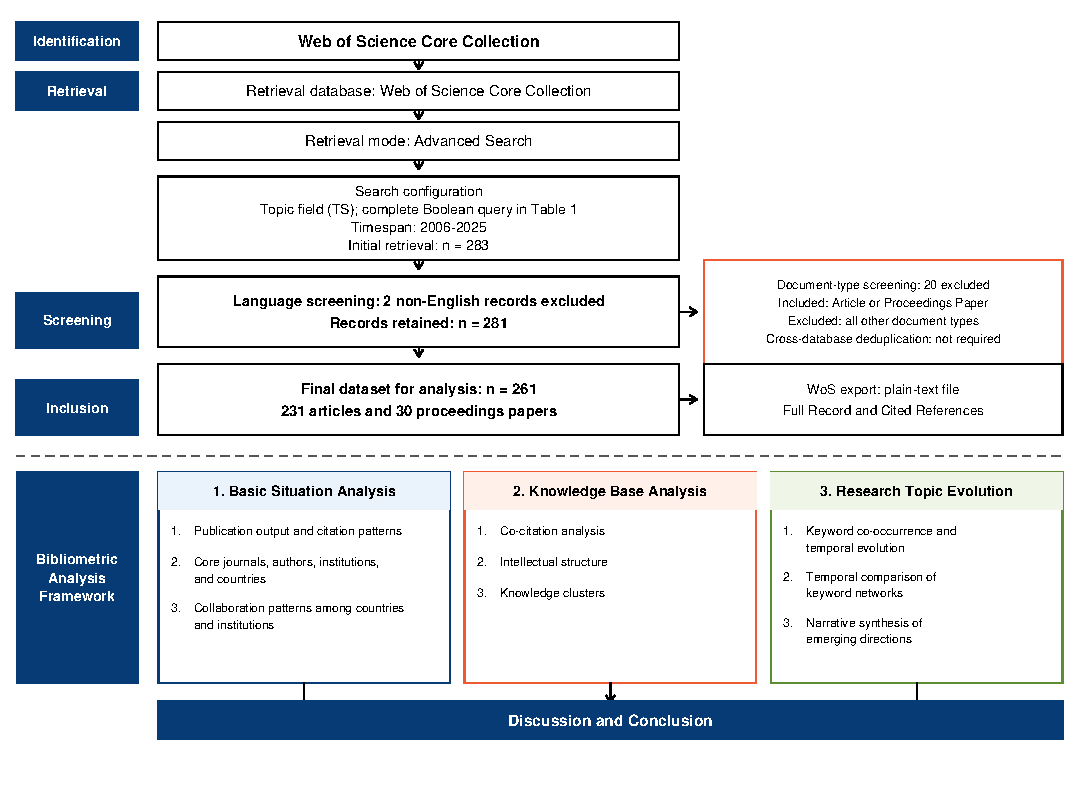
\includegraphics[width=0.9\linewidth]{Figures/flowchart.pdf} 
	\caption{Workflow for literature retrieval, bibliometric analysis, and technical synthesis.}
	\label{fig:flowchart}
\end{figure}


\section{Basic Situation Analysis}
\subsection{Yearly Output}

\begin{figure}[htb!]
	\centering
	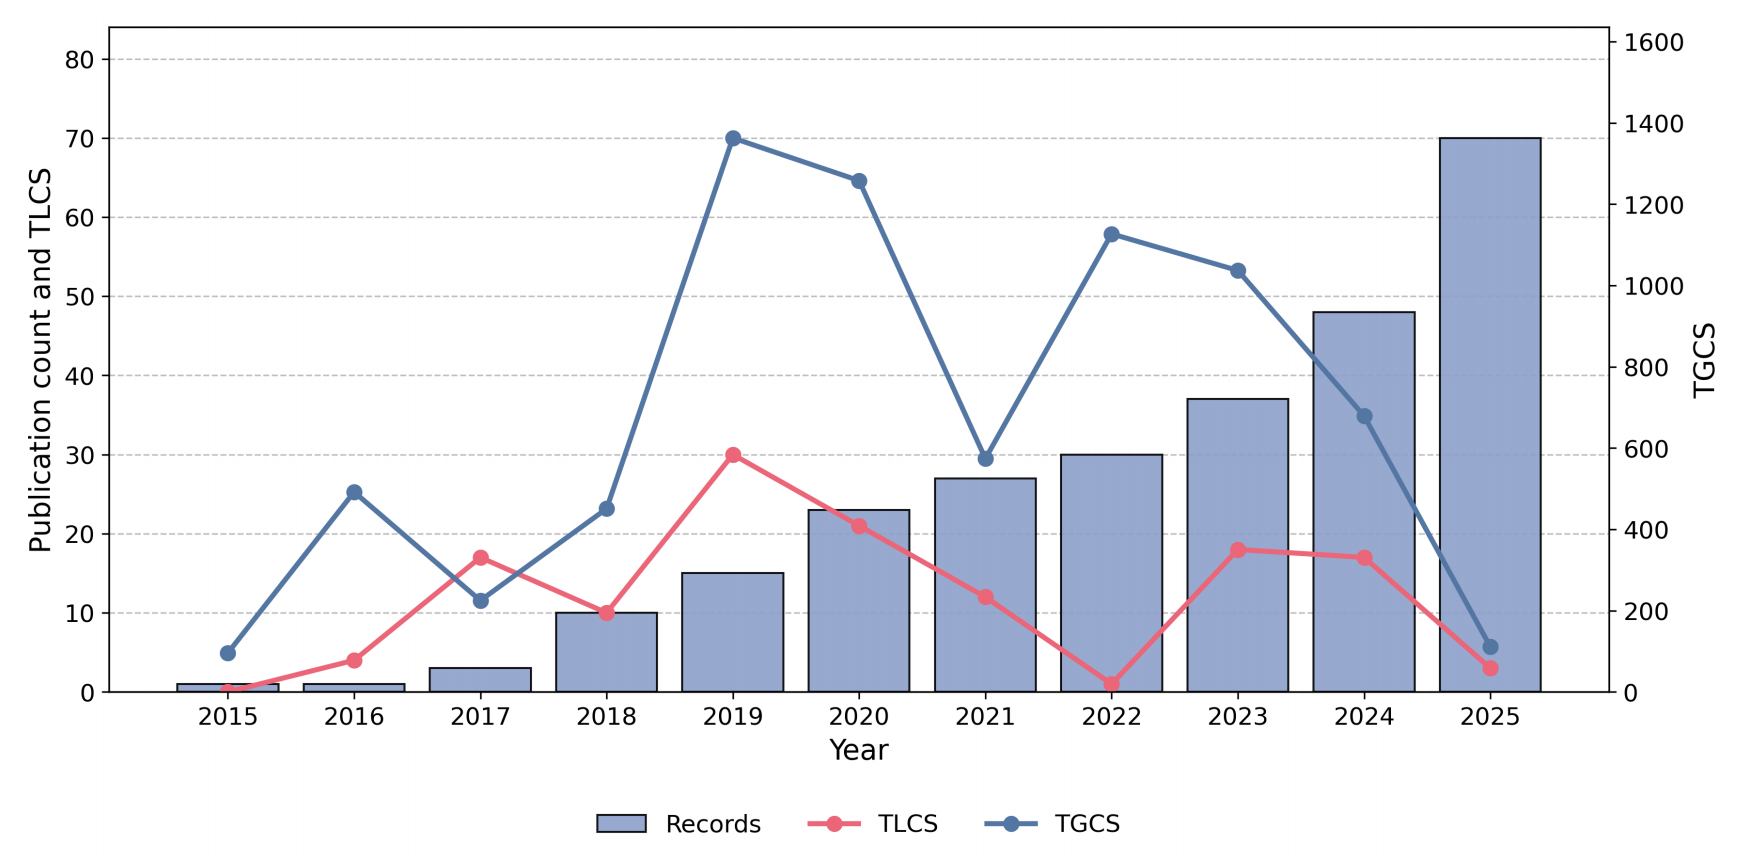
\includegraphics[width=0.75\columnwidth]{picture_2.png}
	\caption{Yearly publication output, TLCS, and TGCS for the retrieved corpus (2015--2025); no records were retrieved for 2006--2014.}
	\label{fig:pub_trends}
\end{figure}

The period 2006--2014 is not explicitly detailed in the figure because no publications were retrieved; however, the single relevant paper published in 2015 is included to mark the onset of research growth. As shown in the figure, the annual volume of publications has exhibited a consistent upward trend. This growth coincided with the rapid advancement of deep learning algorithms and the continuous enhancement of computational power \citep{56}. Notably, the final three years (2023--2025) represent the peak of productivity in the retrieved corpus, with 37, 48, and 70 papers published, respectively. This trend does not establish the share of fusion research in the broader LULC literature.

While publication volume is an indicator of research activity, it does not fully capture academic influence. To address this, TLCS and TGCS based on citation counts are employed to gauge scholarly impact. Notably, TGCS values are generally higher than TLCS, as they encompass citations from the entire Web of Science database rather than just within the selected local dataset \citep{bornmann2011citation}.

TLCS reached its peak in 2019 (30), indicating that papers published in this year have attracted substantial attention within the selected corpus. Analysis reveals that two highly cited papers were the primary contributors to this peak: ``Advanced Multi-Sensor Optical Remote Sensing for Urban Land Use and Land Cover Classification: Outcome of the 2018 IEEE GRSS Data Fusion Contest'' (TLCS=17) \citep{21} and ``Combining Sentinel-1 and Sentinel-2 Satellite Image Time Series for land cover mapping via a multi-source deep learning architecture'' (TLCS=8) \citep{22}. Furthermore, although 2017 had a lower volume of publications, it maintained a relatively high TLCS. This is largely due to the work ``Hyperspectral and LiDAR Data Fusion Using Extinction Profiles and Deep Convolutional Neural Network'' (TLCS=15) \citep{23}. Annual citation totals can be concentrated in a small number of papers and are affected by publication age and citation practices.

TGCS similarly peaked in 2019 (1363), driven by the aforementioned works and complemented by ``Urban Tree Species Classification Using a WorldView-2/3 and LiDAR Data Fusion Approach and Deep Learning'' \citep{26}. A secondary peak in TGCS occurred in 2020 (1258). In this year, ``Cloud removal in Sentinel-2 imagery using a deep residual neural network and SAR-optical data fusion'' \citep{27} contributed 345 global citations. Interestingly, despite a very low publication count in 2016, the year achieved a high TGCS due to the work ``Deep Learning Earth Observation Classification Using ImageNet Pretrained Networks'' \citep{28}, which contributed 492 citations. 

Within this deliberately focused corpus, several highly cited studies concern the intersection of deep learning and multi-source fusion. We also observe local peaks in the 2023 TLCS and 2022 TGCS following minor declines, which may be attributed to the delayed citation window effect \citep{bornmann2011citation}. Conversely, the scores for 2024 and 2025 remain relatively low, as newly published papers typically require several years to accumulate significant citation counts.


\subsection{Core Journals, Authors, Institutions, and Countries}

\subsubsection{Active Journals}


Scientific journals serve as the primary conduits for disseminating research findings and academic activities. The 261 publications analysed in this study were distributed across 81 different journals. The top ten journals ranked by publication count, Total Local Citation Score (TLCS), and Total Global Citation Score (TGCS) are summarised in Fig.~\ref{fig:journal_impact}.
\begin{figure}[htb!] 
	\centering
	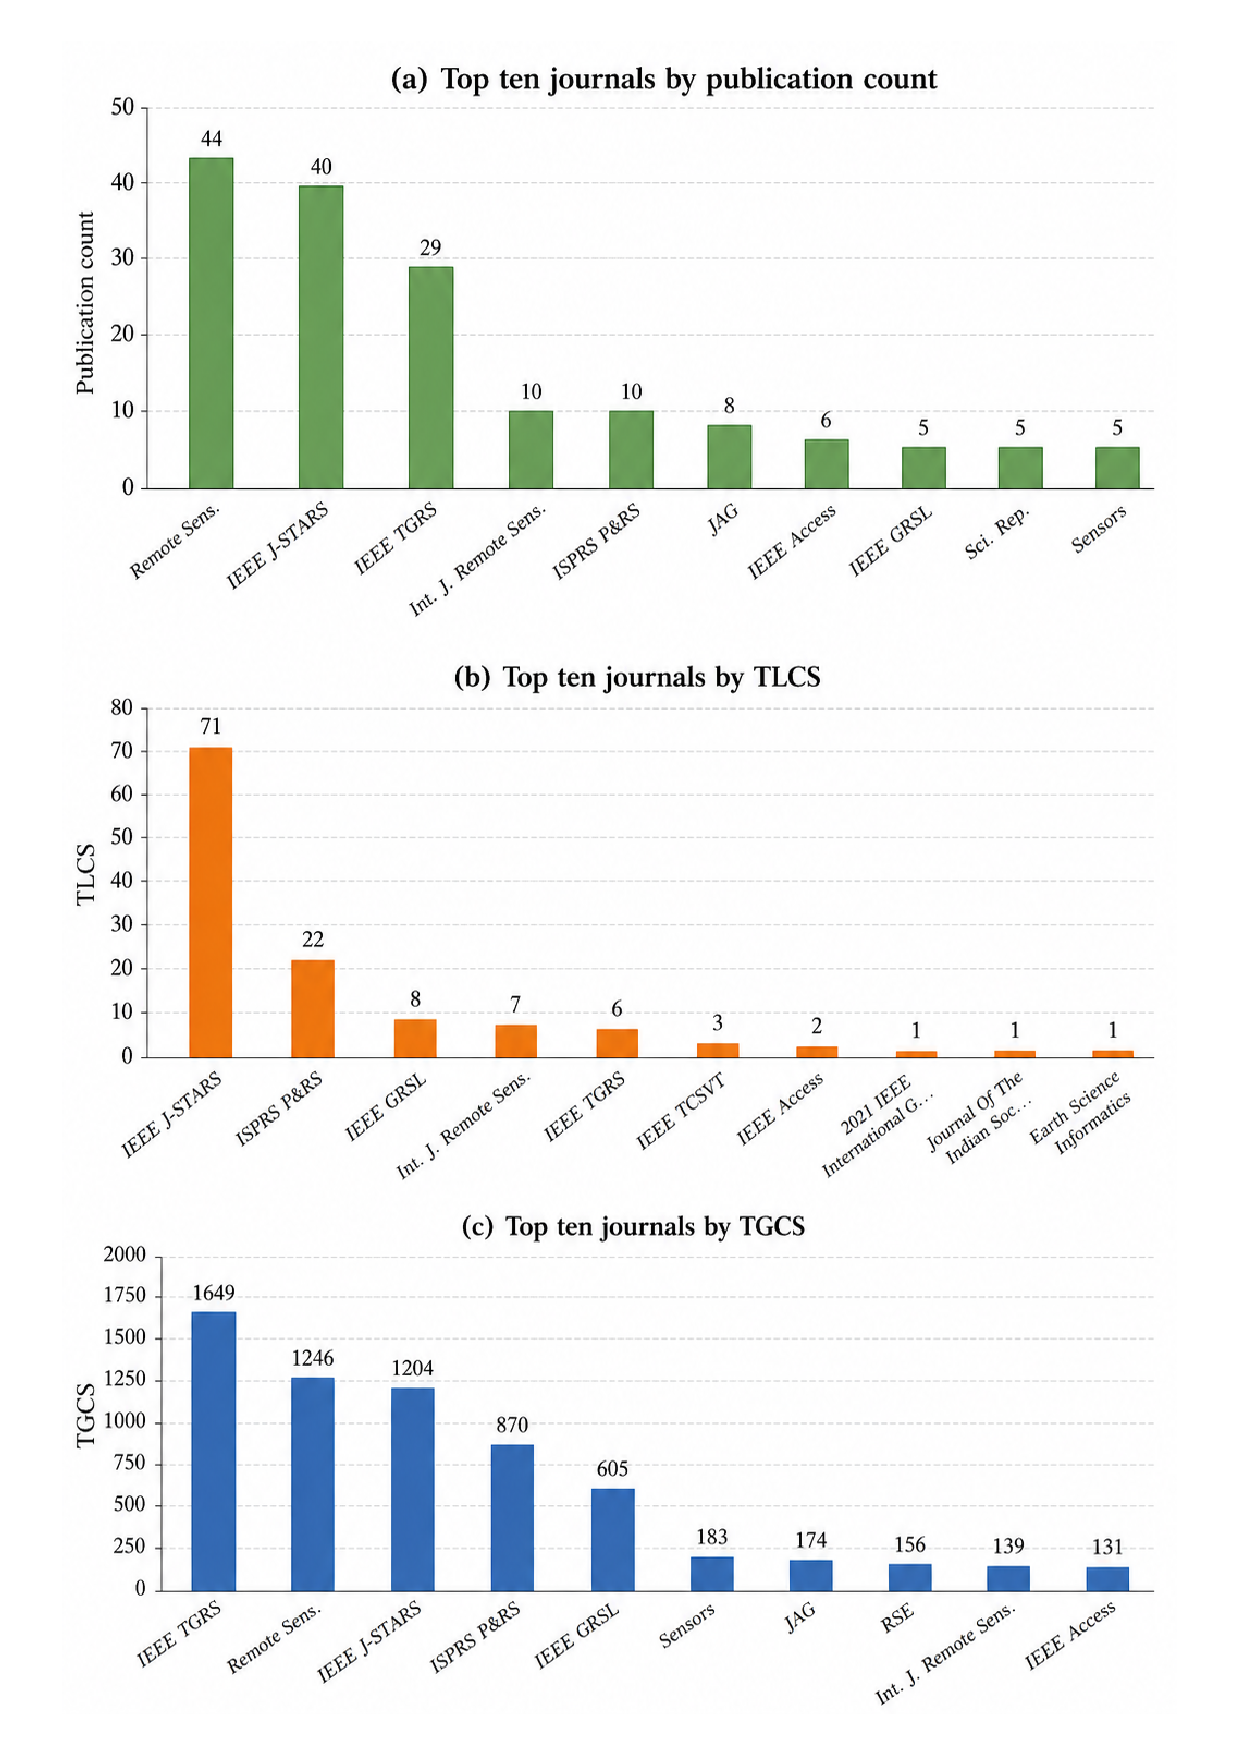
\includegraphics[width=0.67\columnwidth]{Figures/Picture_3.pdf} 
	\caption{Publication count, TLCS, and TGCS per journal (2006--2025).}
	\label{fig:journal_impact}
\end{figure}


According to Fig.~\ref{fig:journal_impact}(a), \textit{Remote Sensing} ranks first in terms of publication volume, making it the most active journal within the retrieved corpus. However, its TLCS (7) only ranks fourth, compared to its TGCS (1246). These indicators use different citation populations; the observed difference does not establish an effect of open access or journal scope.

In contrast, \textit{IEEE J-STARS} ranks first in TLCS and third in TGCS (Fig.~\ref{fig:journal_impact}(b, c)), within the retrieved corpus. Furthermore, \textit{IEEE TGRS} leads in TGCS (1649), although raw citation totals are influenced by publication age and a few highly cited papers.


\subsubsection{Important Authors}

Identifying key authors helps researchers grasp research hotspots and academic trends. In this study, 1,083 authors contributed to the 261 analysed papers. The authors were ranked based on publication count, TLCS, and TGCS, as illustrated in Fig.~\ref{fig:author_impact}. 


\begin{figure}[htb!] 
	\centering
	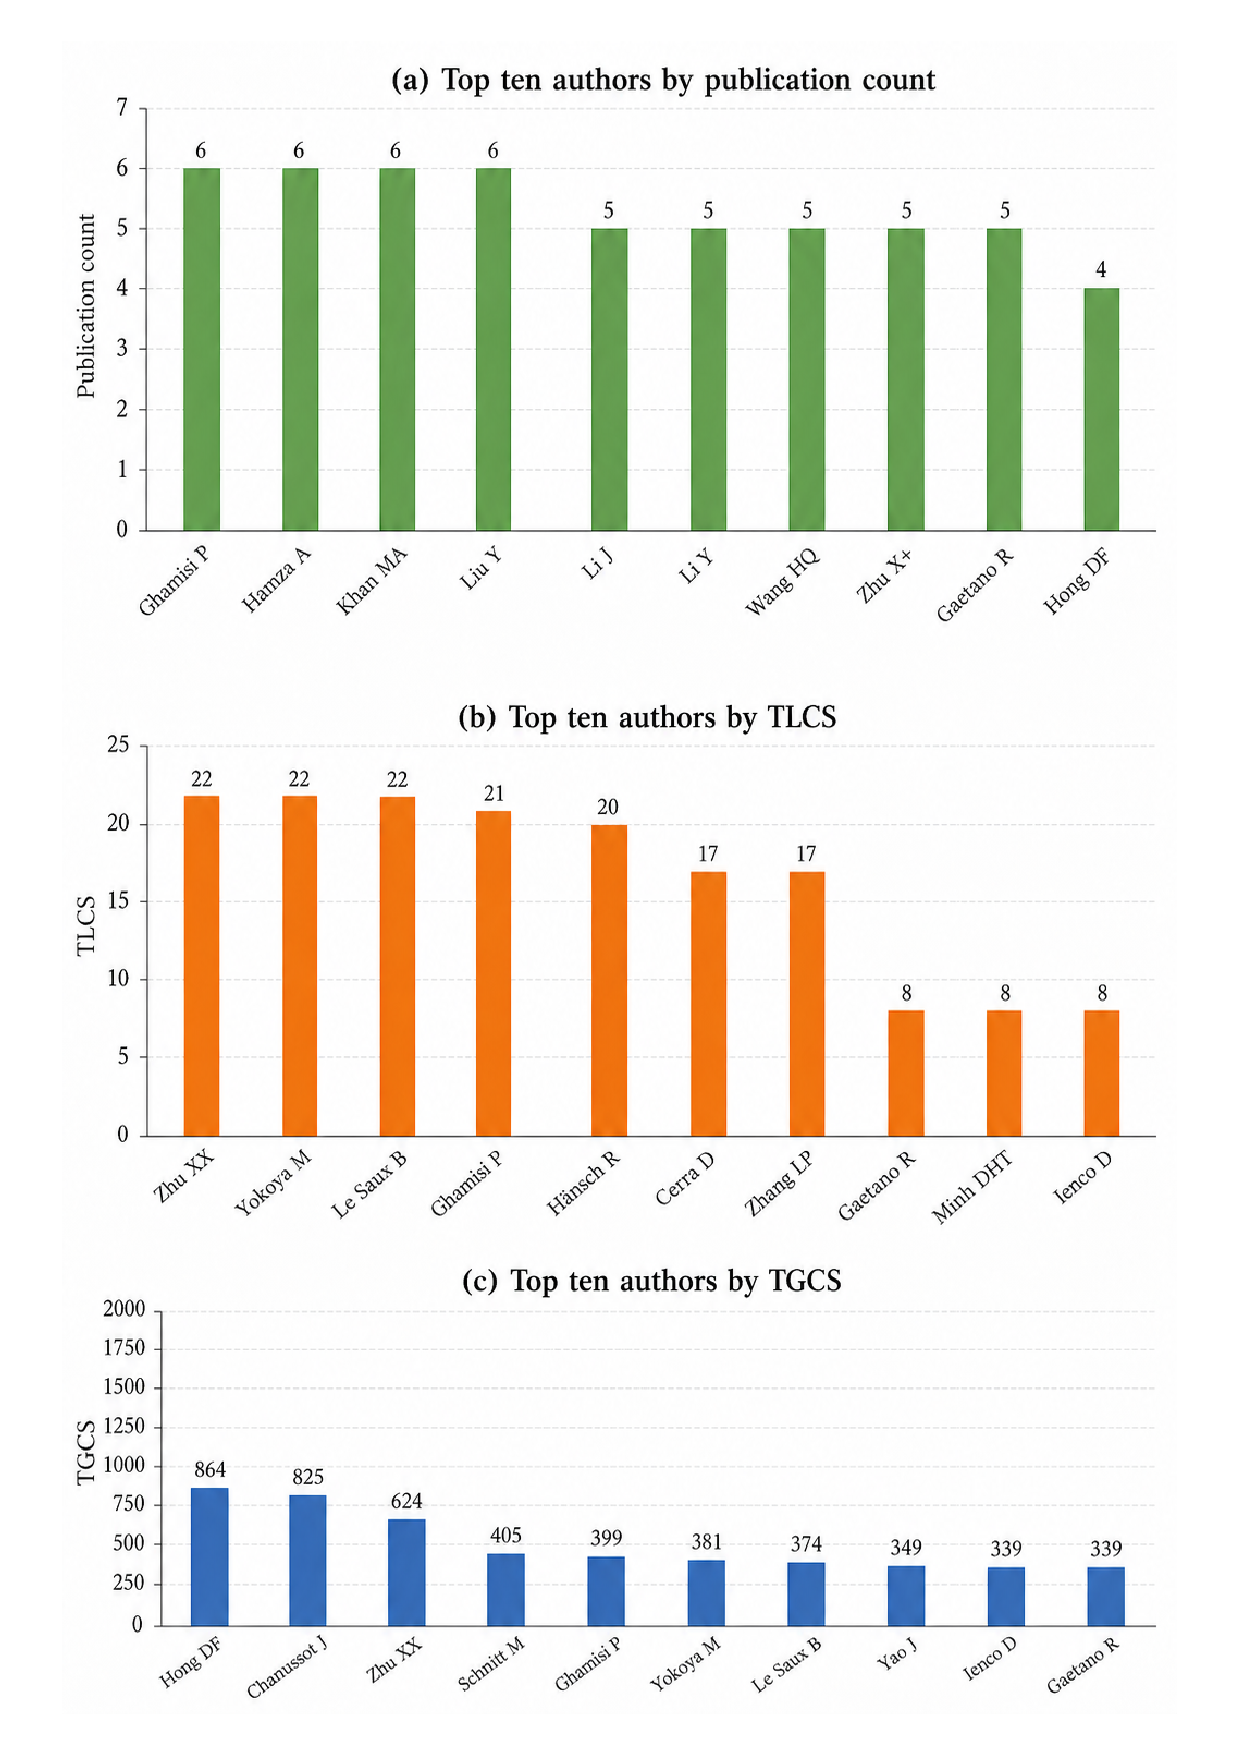
\includegraphics[width=0.67\columnwidth]{Figures/Picture_4.pdf} 
	\caption{Publication count, TLCS, and TGCS per author within the retrieved corpus (2006--2025).}
	\label{fig:author_impact}
\end{figure}

While Ghamisi P., Hamza A., Khan M. A., and Liu Y. lead in publication count with six papers each, further analysis of Fig.~\ref{fig:author_impact} (b, c) reveals that only Ghamisi P. maintains a top-ten ranking in both TLCS (5th, 21) and TGCS (5th, 399). This demonstrates his citation impact within both the local corpus and the wider Web of Science database. Notably, Zhu X. X., Yokoya N., and Le Saux B. also exhibit high TLCS values (22 each). The collaborative work by Ghamisi P. and Zhu X. X., ``Hyperspectral and LiDAR Data Fusion Using Extinction Profiles and Deep Convolutional Neural Network'' \citep{23}, contributed a notable TLCS of 15. Hong D. F. shows the highest TGCS in the retrieved corpus, primarily due to the work of 2022 ``Convolutional Neural Networks for Multimodal Remote Sensing Data Classification'' \citep{2}, which achieved a TGCS of 450.


\subsubsection{Active Institutions and Main Countries}
Institutions play a pivotal role in analysing developmental trends within the retrieved LULC literature. By calculating the affiliations of all authors, a total of 420 institutions were identified. The statistical results for publication volume, Total Local Citation Score (TLCS), and Total Global Citation Score (TGCS) for each institution are summarised in Fig.~\ref{fig:inst_impact}. Wuhan University leads with 24 publications, making it the most active institution within the retrieved corpus. The Chinese Academy of Sciences (CAS) and Huazhong University of Science and Technology follow in second and third place, with 22 and 10 publications, respectively. Notably, the output from Wuhan University and CAS exceeds that of the other listed institutions.


In terms of TLCS rankings, the German Aerospace Center (DLR) and Zhuhai University hold prominent positions. Wuhan University, the Pakistan Institute of Engineering and Applied Sciences (PIEAS), and the University of Technology Sydney follow closely, each with a TLCS of 22. These results indicate that Wuhan University not only maintains high publication output but also receives substantial citation attention within the analysed corpus. Regarding TGCS (as shown in Fig.~\ref{fig:inst_impact}(c)), CAS and Zhejiang University have the highest TGCS values in the retrieved corpus. 


National contribution is another critical dimension for assessing academic activity in LULC. The retrieved literature spans 134 countries. The top ten countries by publication volume account for 89.30\% of the total output. Fig.~\ref{fig:country_impact} illustrates the distribution of the top ten countries across the three metrics: publication count, TLCS, and TGCS. Germany and China rank within the top three across all three metrics. However, raw publication counts do not fully reflect national research intensity; population size, research-system size, database coverage, and publication age can affect these indicators. No normalised comparison of national research capacity was performed. Six countries, including China, Germany, India, France, the UK, and Japan, consistently rank among the top ten across all indicators in this corpus. 


As shown in Figs.~\ref{fig:country_impact} and~\ref{fig:country_collab_compact}, China has the largest publication count in the retrieved corpus. The majority of China's records are single-country publications (indicated by the large light-green portion in Fig.~\ref{fig:country_collab_compact}), while multi-country collaborative papers represent a smaller fraction. This spatial distribution is further elucidated in Fig.~\ref{fig:collab_map}, which visualises the intensity and geographical direction of these partnerships. Collaborative links extend from China to countries in North America, Europe, and Australia within this corpus.

Other countries exhibit distinct collaboration patterns: India and Germany also show a high proportion of single-country publications. In contrast, while the total publication volumes for the USA, South Korea, Iran, and Australia decrease sequentially, their proportion of international collaborative papers (indicated in red in Fig.~\ref{fig:country_collab_compact}) is more prominent. As illustrated in the geographical distribution (Fig.~\ref{fig:collab_map}), these nations have international collaborative links. These patterns describe co-authorship in the selected corpus and do not establish that collaboration increased research quality or citation impact.

\begin{figure}[!htbp]
	\centering
	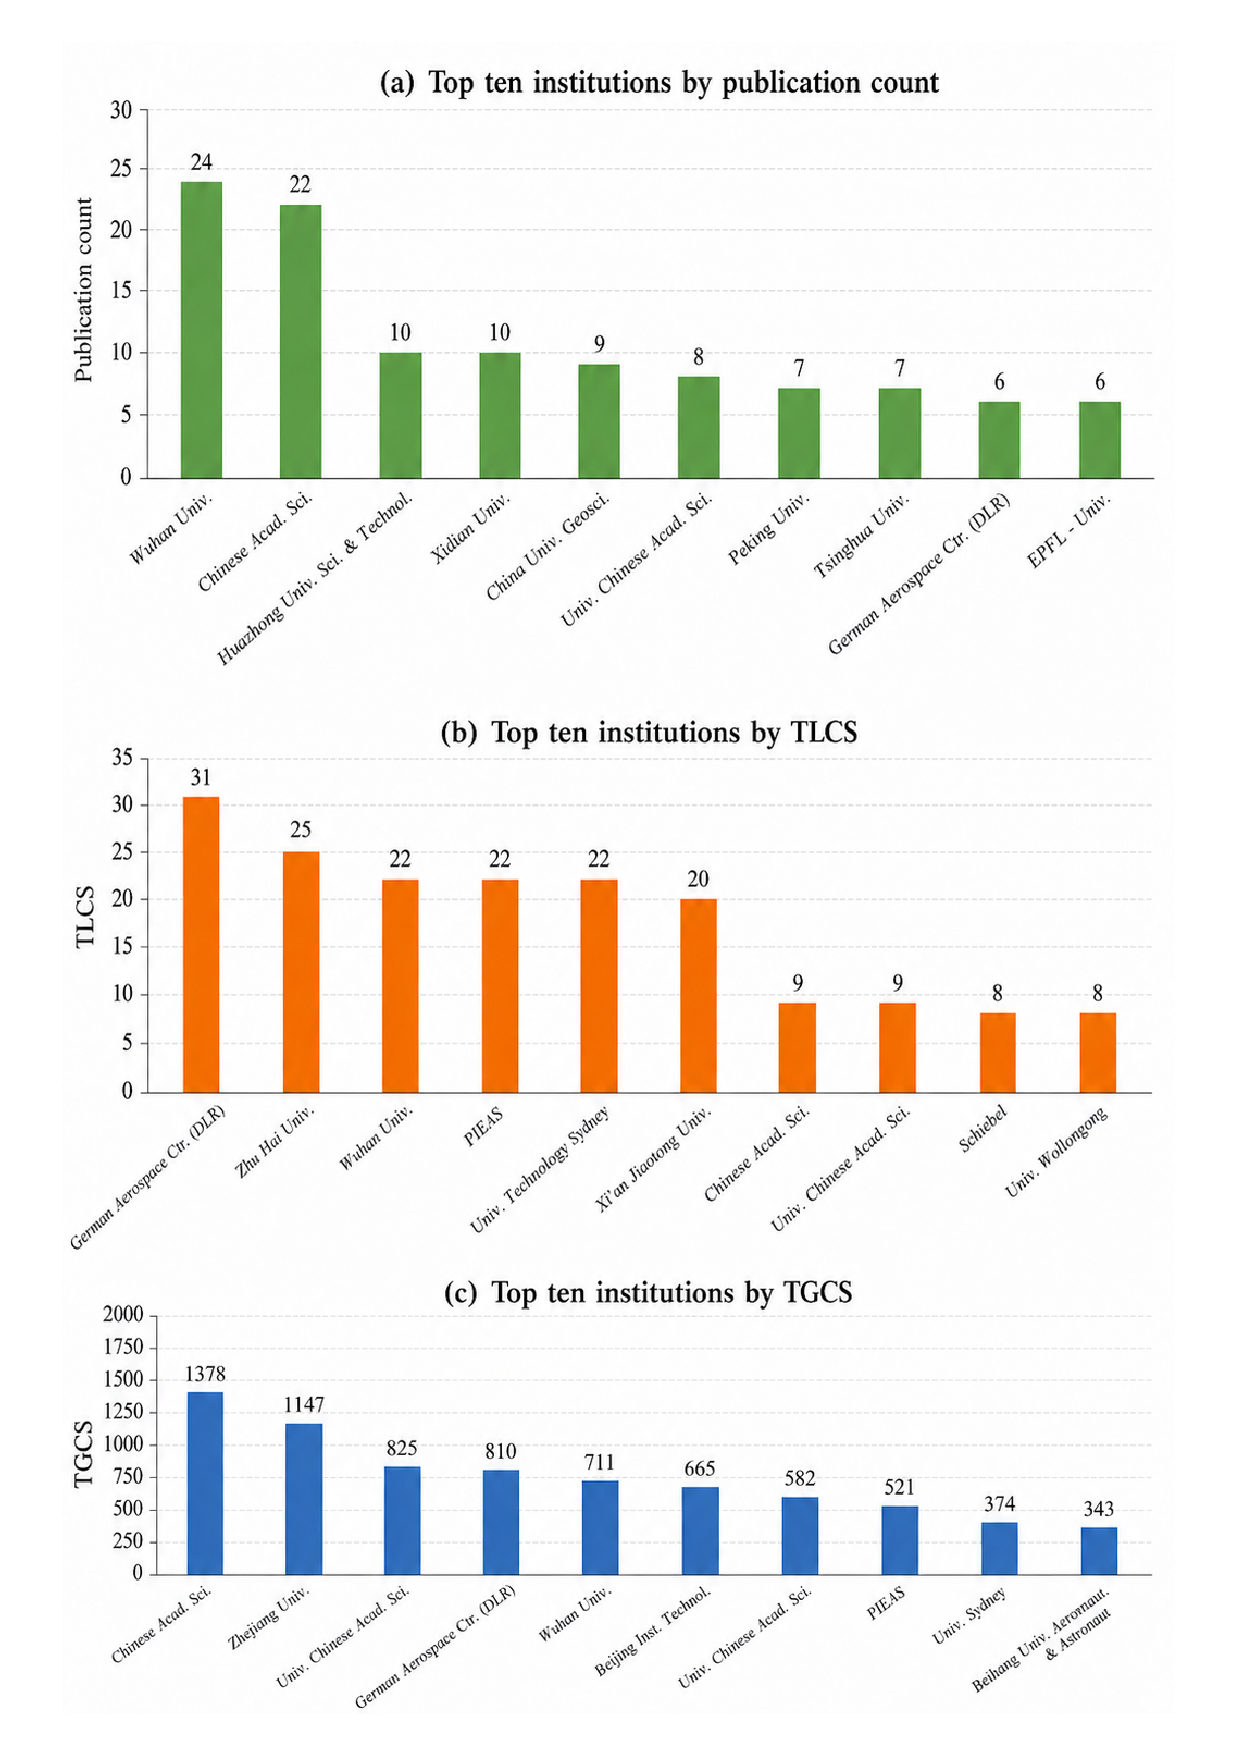
\includegraphics[width=0.67\columnwidth]{Figures/Picture_5.pdf} 
	\caption{Publication volume, TLCS, and TGCS per institution within the retrieved corpus (2006--2025).}
	\label{fig:inst_impact}
\end{figure}


\begin{figure}[!htbp]
	\centering
	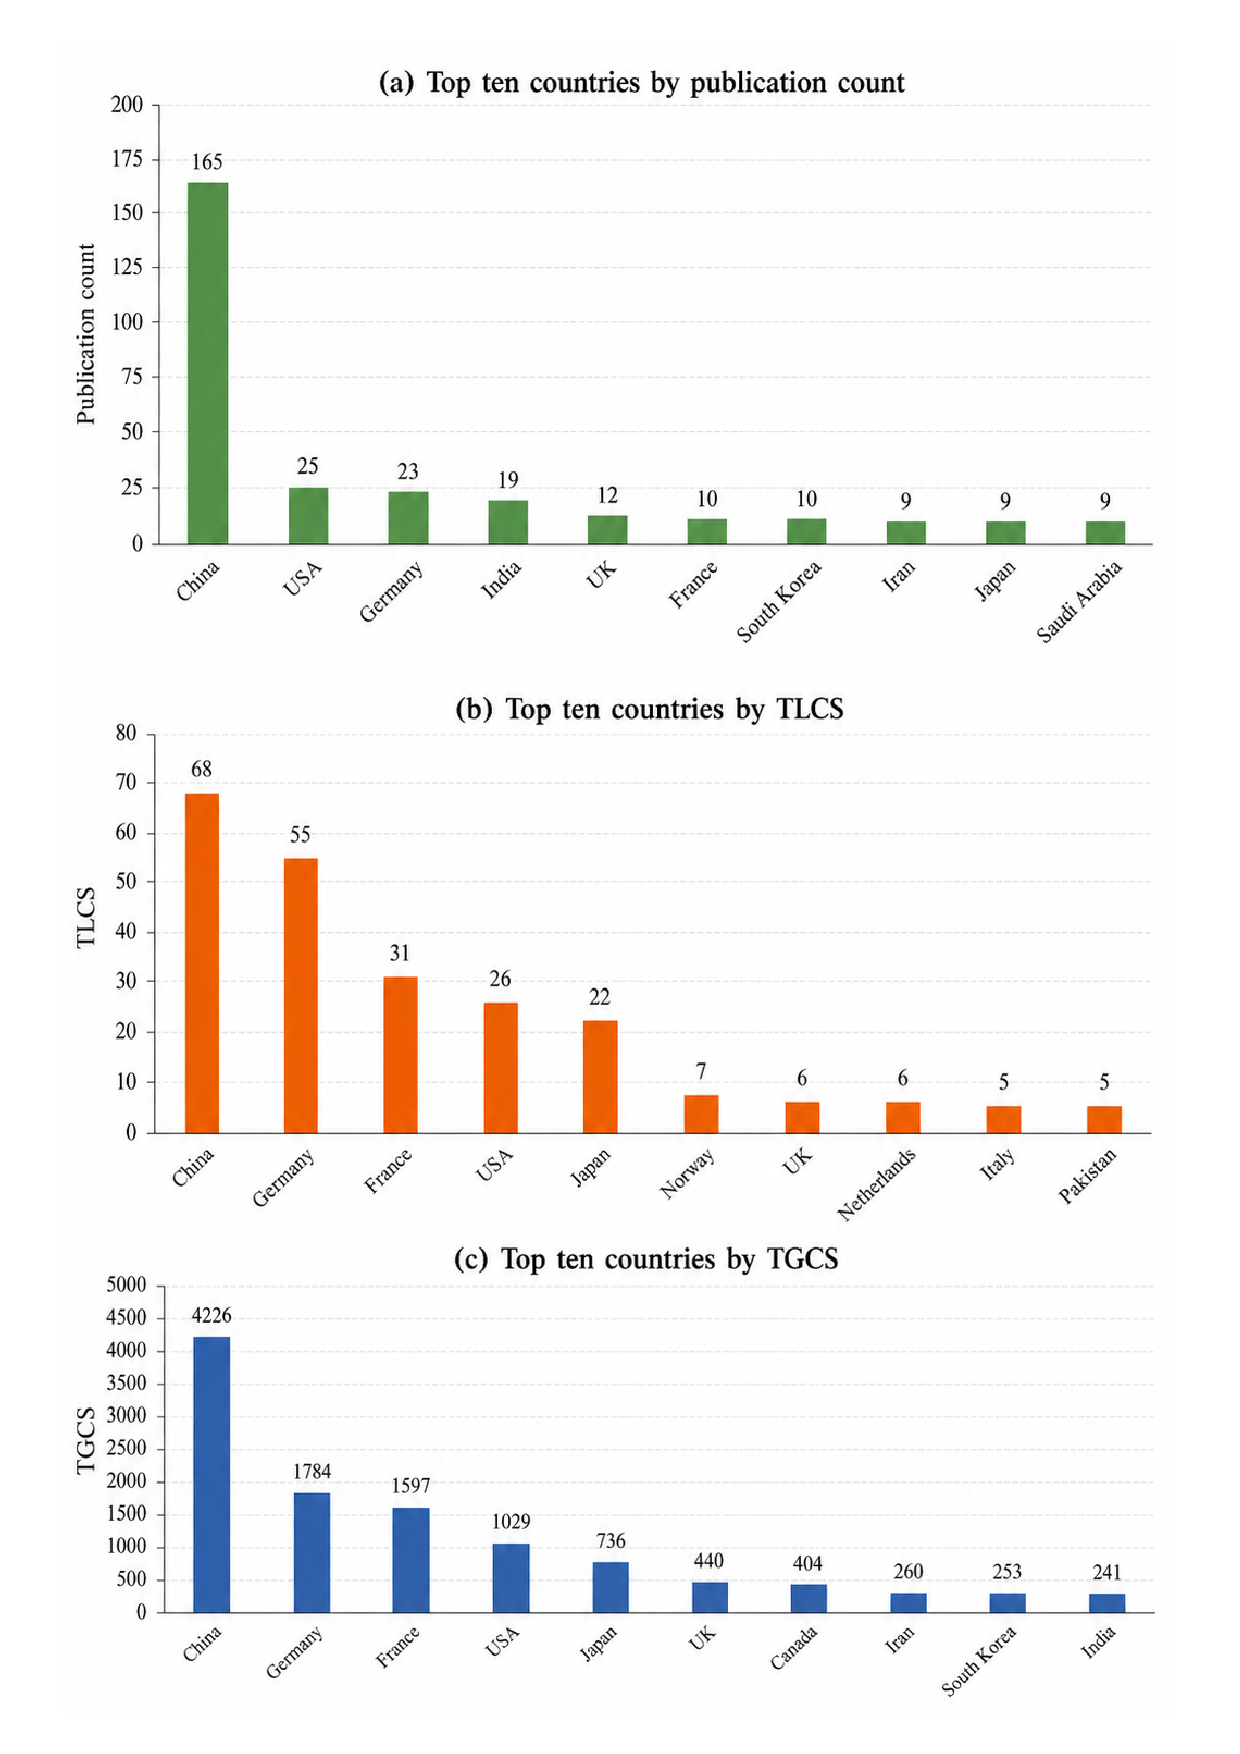
\includegraphics[width=0.67\columnwidth]{Figures/Picture_6.pdf} 
	\caption{Top ten countries ranked by publication volume, TLCS, and TGCS within the retrieved corpus (2006--2025).}
	\label{fig:country_impact}
\end{figure}

\begin{figure}[htb!]
	\centering	
	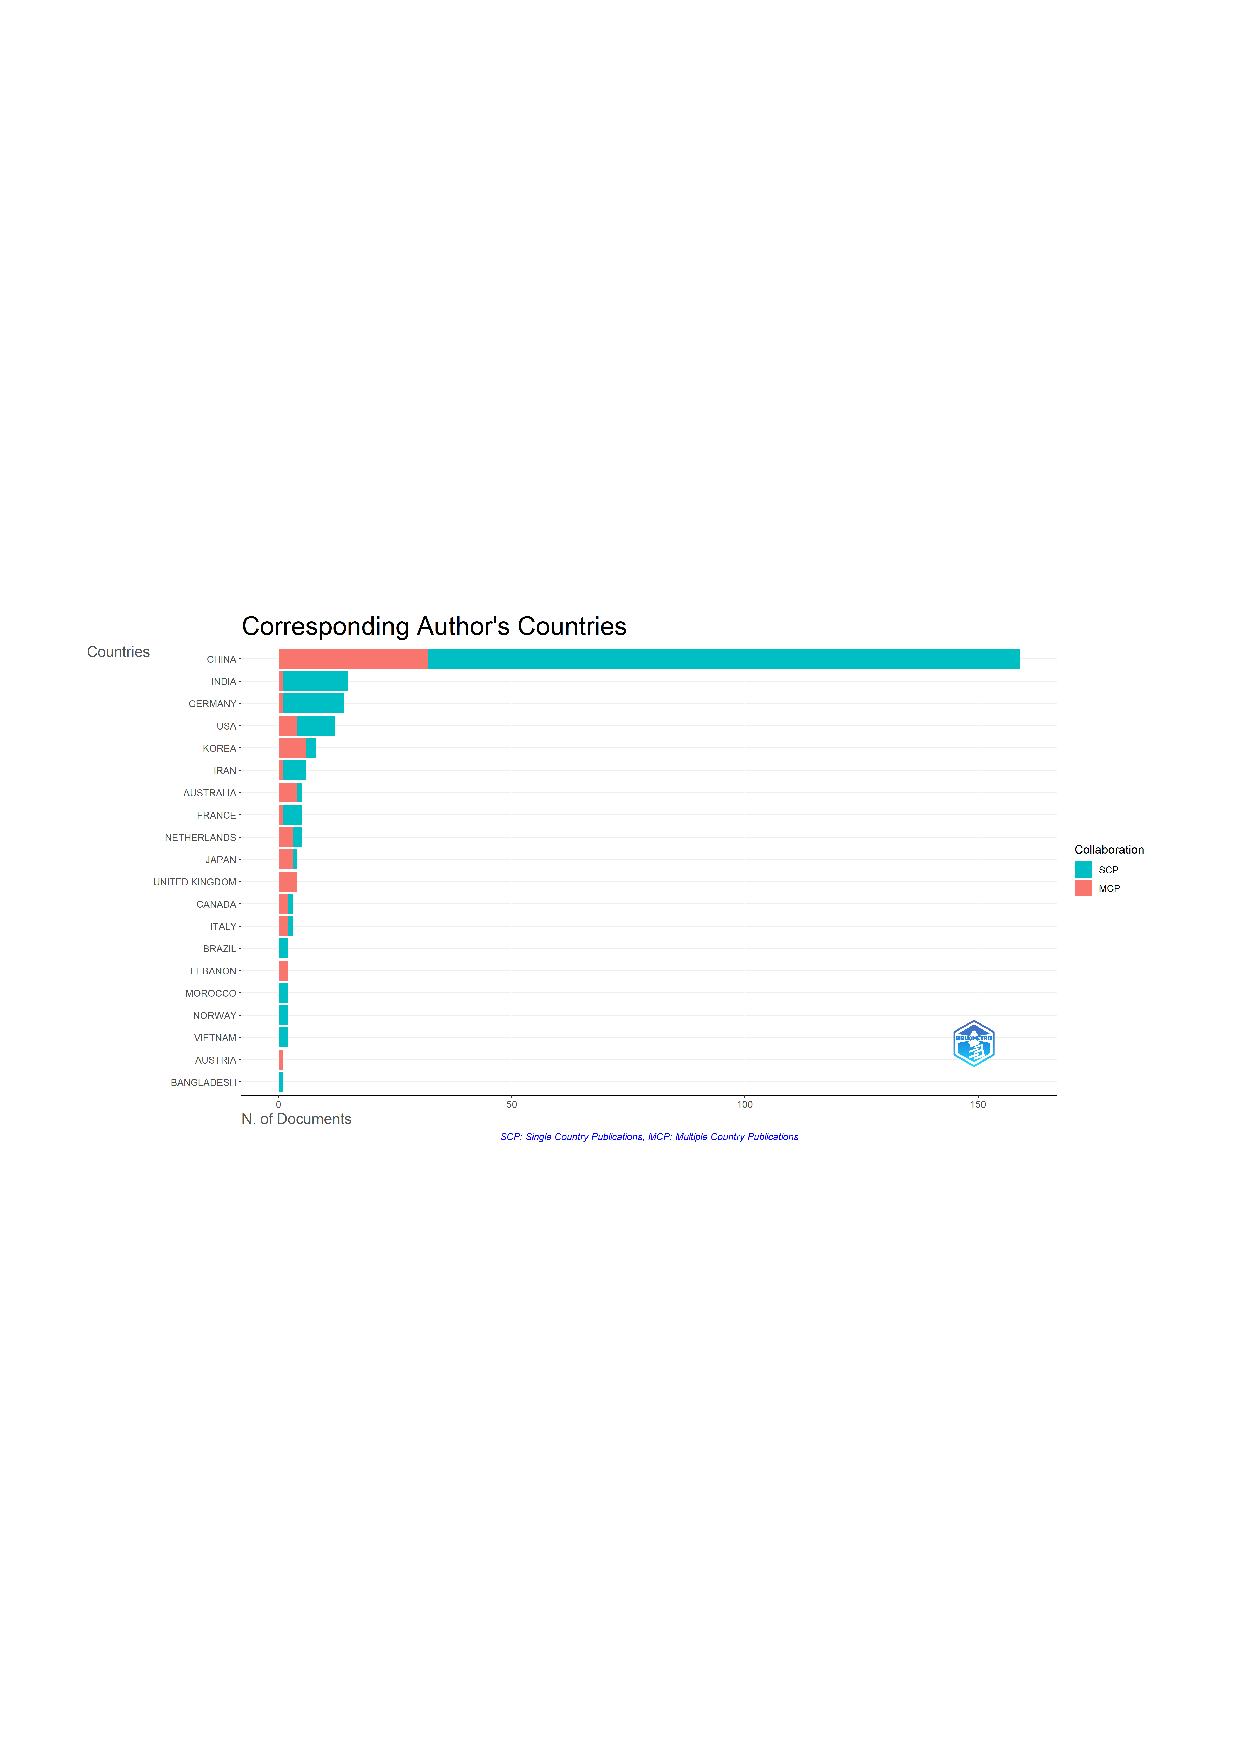
\includegraphics[width=1.0\textwidth, height=0.38\textheight, keepaspectratio]{Figures/picture_7.pdf}
	\vspace{-10pt}
	\caption{Collaboration analysis of major countries: MCP versus SCP. Here, MCP denotes Multiple Country Publication (i.e., co-authors from two or more different countries), while SCP denotes Single Country Publication (i.e., all authors affiliated with the same country).}
	\label{fig:country_collab_compact}
	\vspace{10pt}
	
	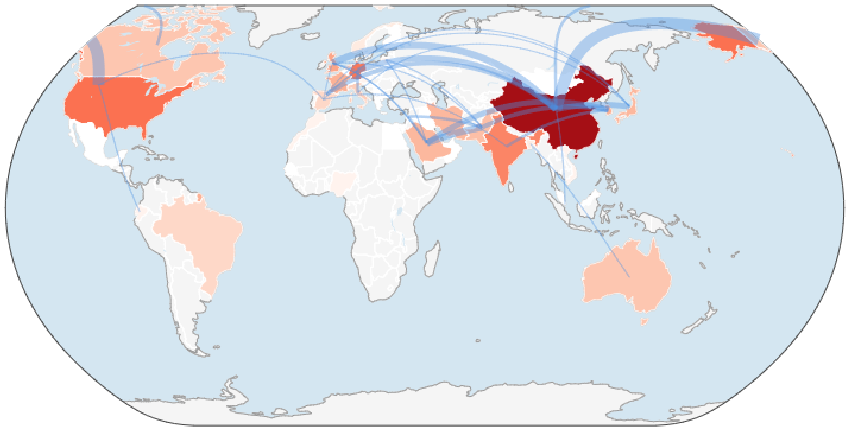
\includegraphics[width=\linewidth]{Figures/newplot_original_pdf_fig8.pdf}
	\vspace{-10pt}
	\caption{Geographical distribution of international research collaborations. Country shading indicates publication output within the retrieved corpus, with darker red indicating more publications. Blue lines represent international co-authorship links, with thicker lines indicating more co-authored publications between the connected countries.}
	\label{fig:collab_map}
\end{figure}

\section{Results and Discussion}

\subsection{Keyword Co-occurrence and Temporal Evolution}

In this study, VOSviewer software was employed to conduct a keyword hotspot analysis on 261 publications related to LULC classification indexed in the Web of Science database from 2006 to 2025. The analysis reveals the core research trends and their temporal evolution within the retrieved corpus, as illustrated in Fig.~\ref{fig:keyword_evolution}. Notably, because no records were retrieved for 2006--2014 and only one for 2015, keyword visualisation for that specific decade is omitted.

\begin{figure}[!htbp]
	\centering
	\subfloat[2016--2020]{%
		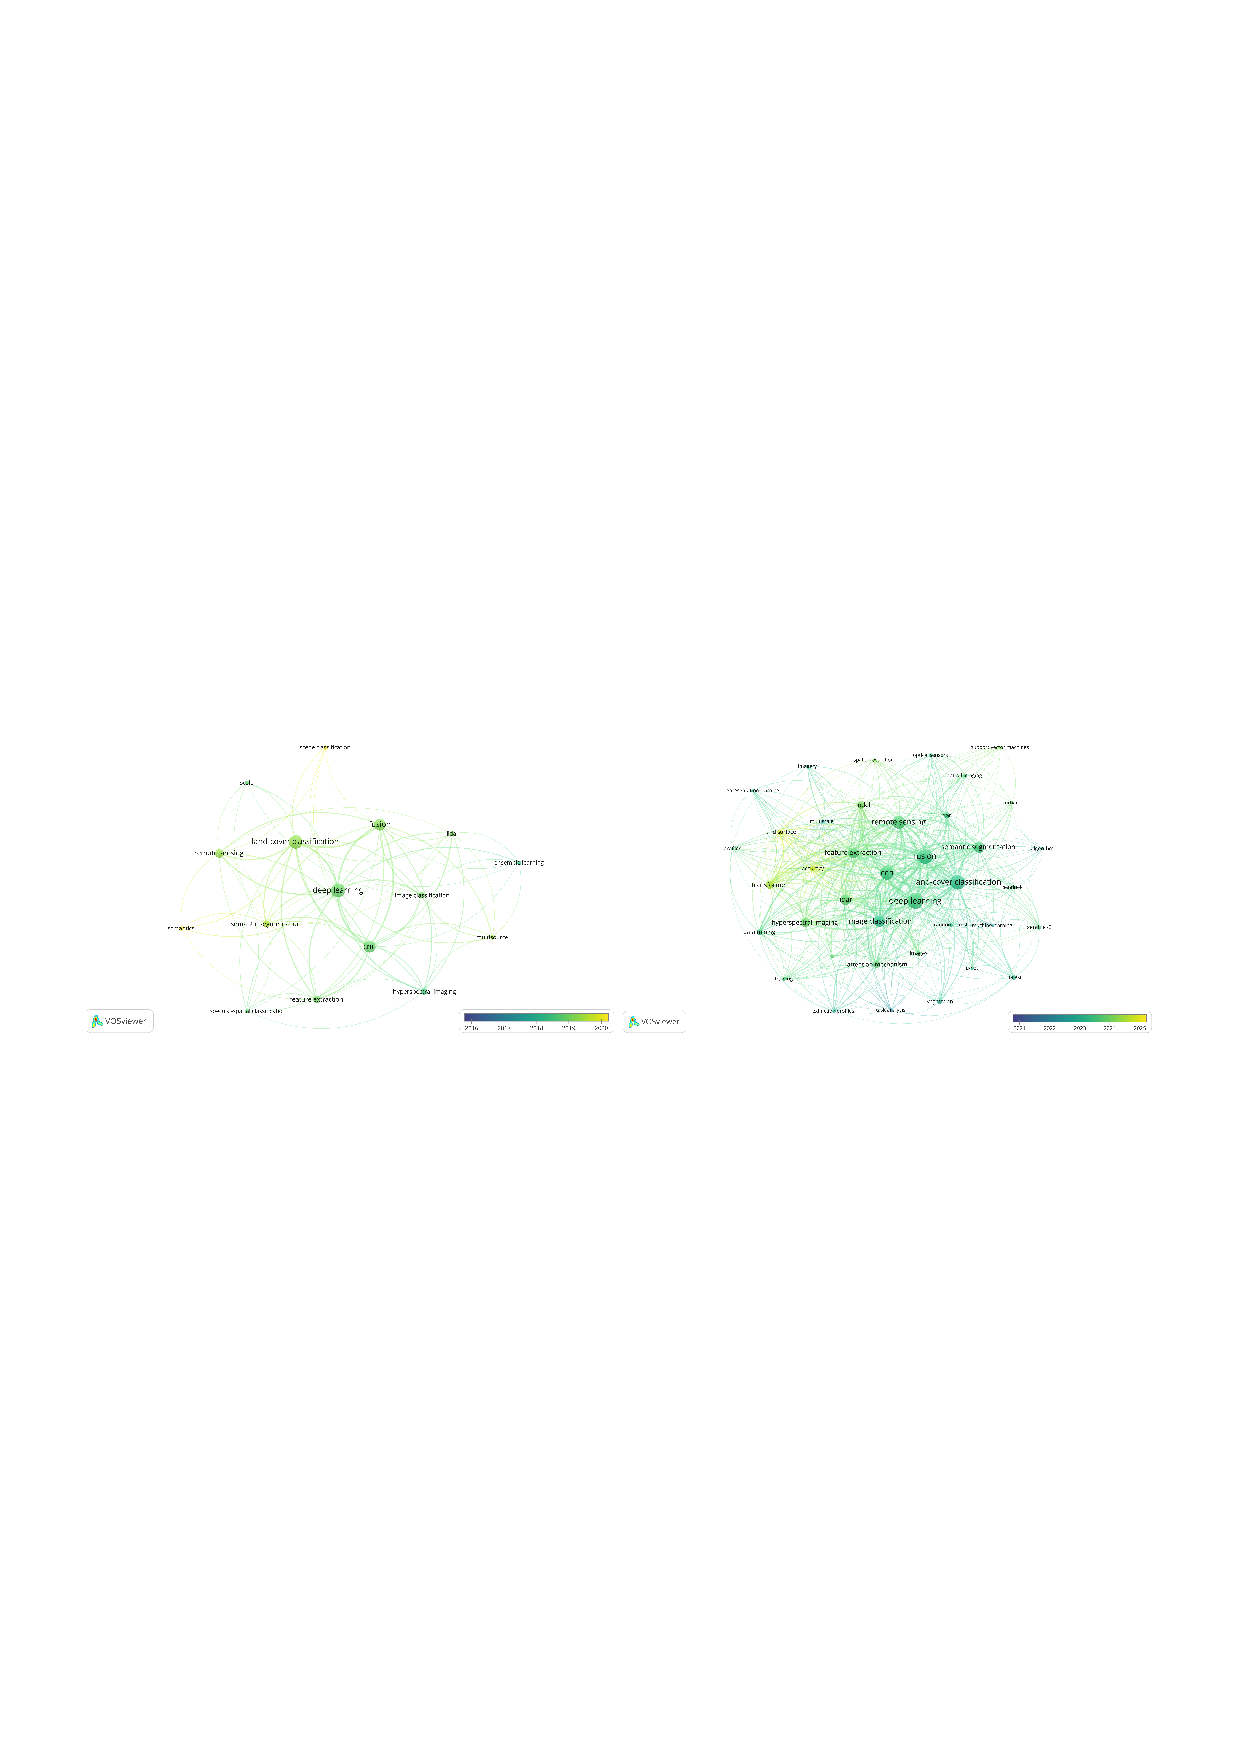
\includegraphics[
			width=0.96\linewidth,
			trim=0 0 256 0,
			clip
		]{Figures/picture_8.pdf}}
	\par\vspace{8pt}
	\subfloat[2021--2025]{%
		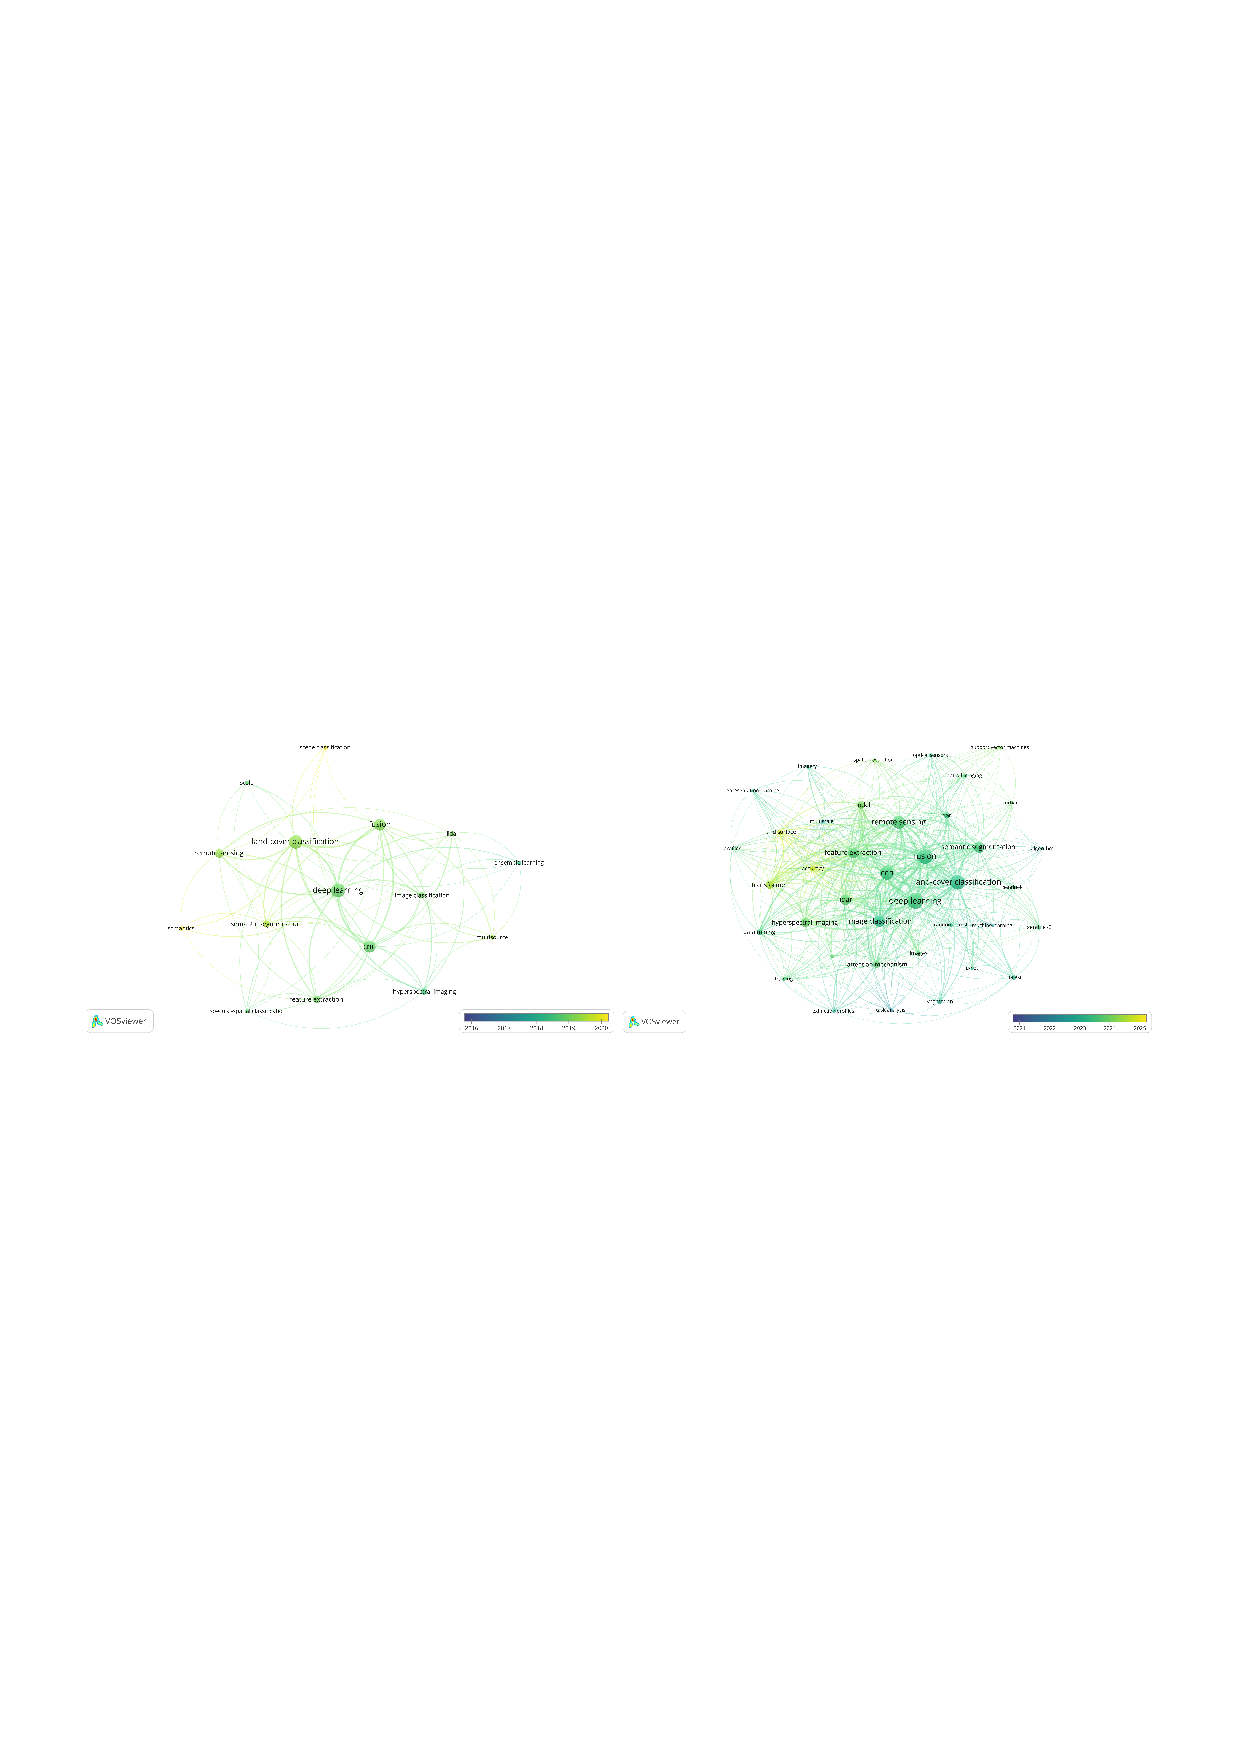
\includegraphics[
			width=0.96\linewidth,
			trim=256 0 0 0,
			clip
		]{Figures/picture_8.pdf}}
	\caption{Keyword co-occurrence networks for the retrieved LULC classification literature: (a) 2016--2020; (b) 2021--2025. Association-strength normalisation and the VOSviewer clustering algorithm were used, with a resolution parameter of 1.00 and a minimum cluster size of 1. Colours indicate average publication year. For readability, labels are displayed only for the more prominent nodes selected by the visualisation software; all retained nodes contribute to network construction.}
	\label{fig:keyword_evolution}
\end{figure}

\begin{figure}[!htbp]
	\centering
	\includegraphics[width=0.98\linewidth]{Figures/new_all.pdf}
	\caption{Keyword co-occurrence network for the retrieved LULC classification literature (2006--2025). Each node represents a keyword, with larger nodes indicating higher occurrence frequencies. Links indicate keyword co-occurrence relationships, and colours indicate clusters. Association-strength normalisation and the VOSviewer clustering algorithm were used, with a resolution parameter of 1.00 and a minimum cluster size of 1. For readability, labels are displayed only for the more prominent nodes selected by the visualisation software; all retained nodes contribute to network construction.}
	\label{fig:keyword_all}
\end{figure}

As shown in Fig.~\ref{fig:keyword_evolution}, during the 2016--2020 period (upper panel), the focus of the retrieved LULC classification research was concentrated on keywords such as ``land-cover classification'', ``deep learning'', ``fusion'', and ``CNN''. These keywords recorded occurrences of 33, 30, 23, and 23, respectively, with their Total Link Strength (TLS) ranking highest at 101, 84, 72, and 72. These terms indicate attention to multi-source data fusion and deep learning within the selected corpus \citep{23,6}; their frequencies do not establish technical superiority or replacement.

According to the analysis of the 2021--2025 period (lower panel of Fig.~\ref{fig:keyword_evolution}), several terms occur more frequently within the retrieved corpus. The occurrences for ``deep learning'', ``fusion'', and ``CNN'' were 104, 94, and 83, with their TLS reaching 422, 422, and 399, respectively. The ``remote sensing'' node also appears prominently with 69 occurrences and a TLS of 351, within the later-period network. Similarly, the ``land-cover classification'' node remains highly conspicuous, indicating continuing attention within the retrieved corpus \citep{cao2020urban}. TLS depends on the size and structure of each period-specific network; values from independently constructed networks should not be interpreted as directly comparable measures of technological progress or performance.

To gain a more holistic perspective, Fig.~\ref{fig:keyword_all} presents the comprehensive keyword co-occurrence network across the entire study period. The dense interconnection between ``deep learning'' and various sensor-specific nodes, such as ``hyperspectral imaging'', ``LiDAR'', and ``SAR'' indicates co-occurrence within this focused literature. Notably, emerging keywords like ``Transformer'', ``attention mechanism'', and ``Mamba'' are also present within the network. Their presence indicates research attention, not superiority over earlier methods.

In contrast, nodes representing traditional methods and sensor terms, such as ``support vector machines'', ``optical sensors'', and ``random forest'' \citep{belgiu2016random}, are smaller in the displayed network. This describes their occurrence in the selected deep-learning-and-fusion corpus, not declining use across LULC research. Colours in the temporal overlay in Fig.~\ref{fig:keyword_evolution} indicate average publication year rather than performance or research quality. Nodes related to multi-source data fusion remain prominent; ``representation learning'' and ``self-attention'' also indicate topics investigated within the corpus.

\FloatBarrier
\subsection{Intellectual Structure}
To reveal the theoretical foundations and intellectual origins of this field, a document co-citation network was constructed using VOSviewer, as illustrated in Fig.~\ref{fig:intellectual_structure}. Co-citation analysis identifies relationships between documents based on their simultaneous citation patterns; it does not directly measure technical performance.

The co-citation network was normalised using the association-strength method. Clusters were identified using the VOSviewer clustering algorithm with a resolution parameter of 1.00 and a minimum cluster size of 1. Each node represents a cited reference, with larger nodes indicating higher citation counts. Links represent co-citation relationships, with greater link strength indicating more frequent co-citation; shorter distances generally indicate closer relationships within the network. Colours denote the clusters identified from the co-citation structure. These clusters are treated as interconnected structural groupings rather than mutually exclusive research themes.

The results reveal four distinct clusters, representing groups of references cited together in the retrieved corpus \citep{19}:

\begin{figure}[!htbp]
	\centering
	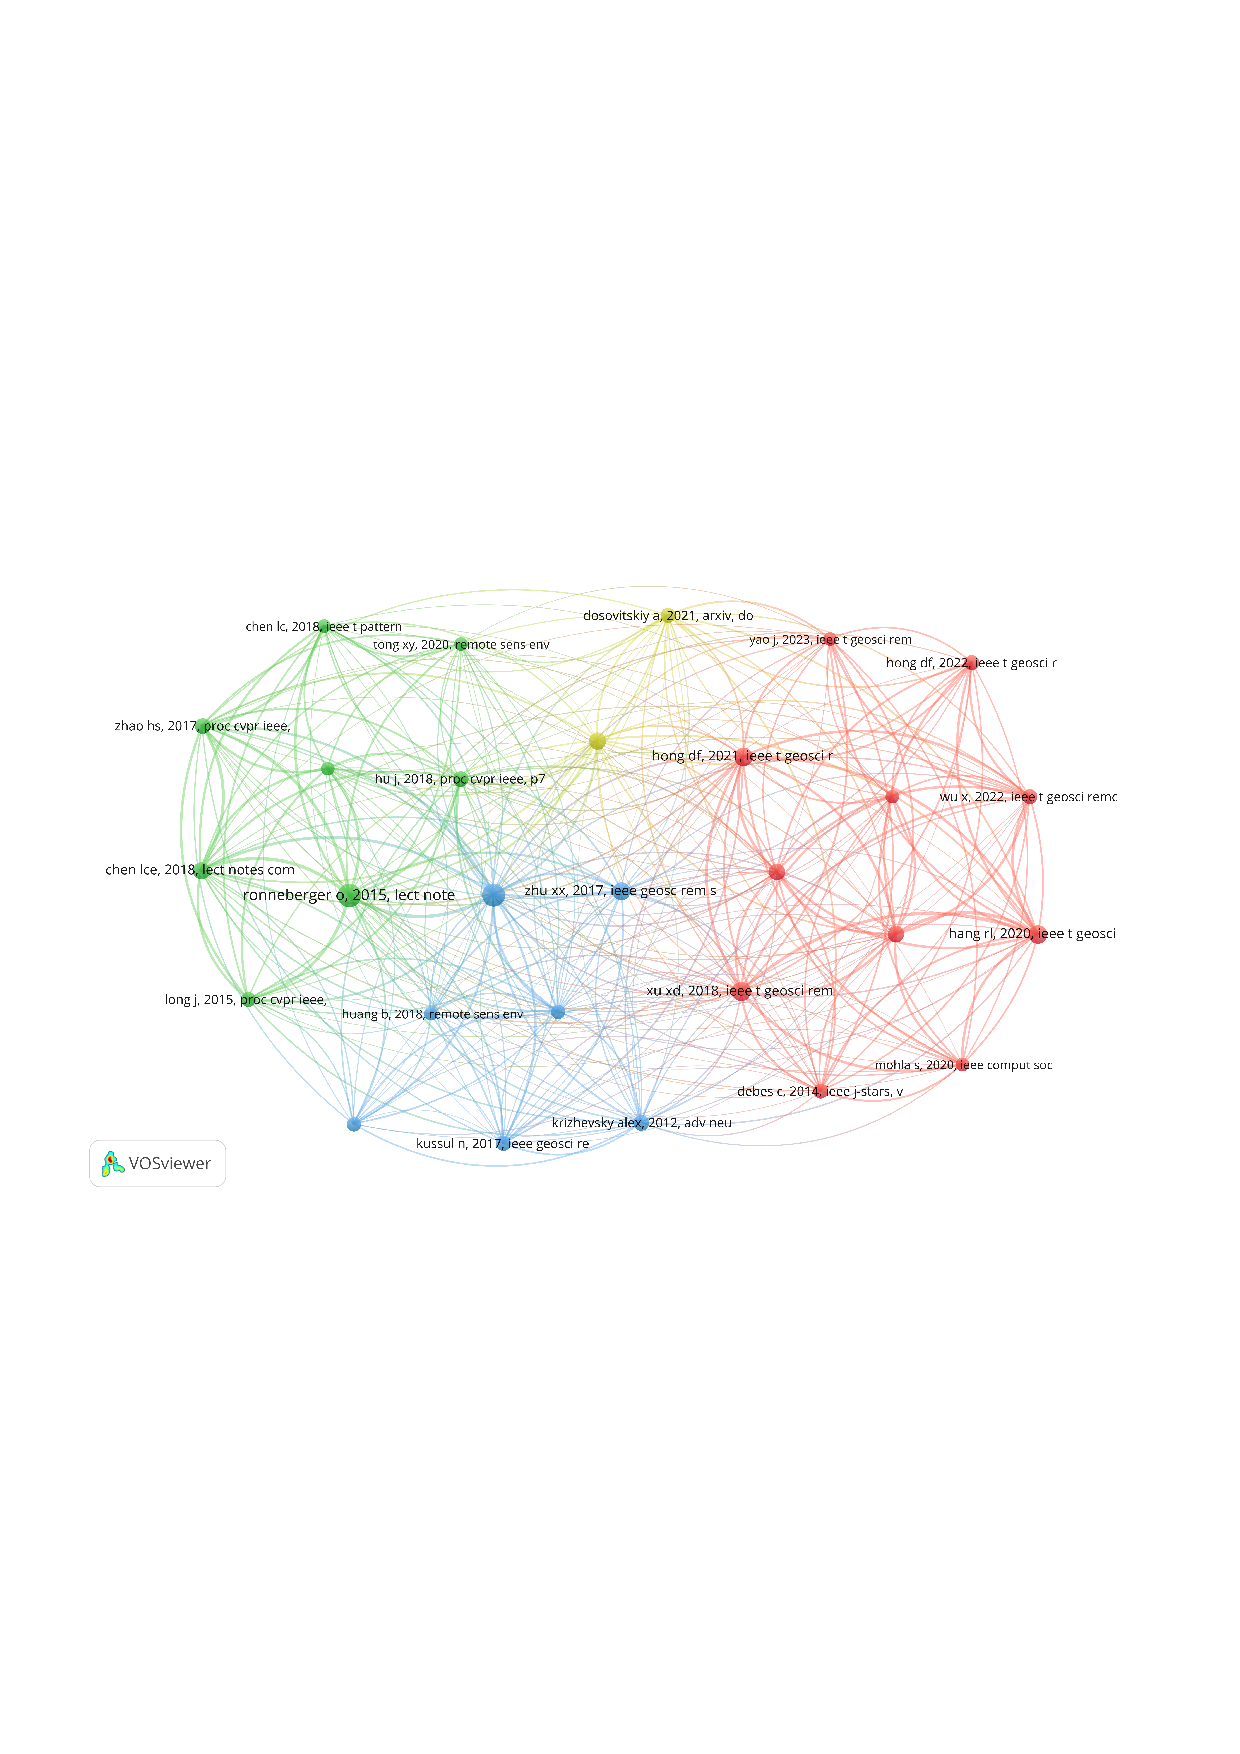
\includegraphics[width=0.98\linewidth]{Figures/picture_9.pdf}
	\caption{Document co-citation network revealing the intellectual structure of the retrieved LULC classification literature. Each node represents a cited reference, with larger nodes indicating higher citation counts within the retrieved corpus. Links indicate co-citation relationships, and colours indicate clusters. Association-strength normalisation and the VOSviewer clustering algorithm were used, with a resolution parameter of 1.00 and a minimum cluster size of 1. For readability, labels are displayed only for the more prominent nodes; all retained nodes contribute to network construction.}
	\label{fig:intellectual_structure}
\end{figure}

\begin{enumerate}
	\item \textbf{Deep Learning Fundamentals (Blue Cluster):} This cluster represents the cornerstone of computer vision algorithms. Core nodes include Krizhevsky et al. (2012, AlexNet) and Simonyan and Zisserman (2015, VGG) \citep{31, 32}. These landmark studies introduced the AlexNet architecture and VGG network, respectively. Although originating from general computer vision, they provided the foundational CNN architectures that serve as primary feature extractors for remote sensing imagery. The work by Marmanis et al. (2016) directly bridges this cluster with remote sensing, marking the successful transfer of ImageNet pre-trained models to Earth observation tasks.
	
	\item \textbf{Semantic Segmentation Paradigm (Green Cluster):} This cluster focuses on ``pixel-to-pixel'' classification methods, which are critical for LULC mapping. Key nodes include Long et al. (2015, FCN) \citep{33} and Ronneberger et al. (2015, U-Net) \citep{34}. These studies established the ``encoder-decoder'' architecture, enabling end-to-end dense prediction. In the context of LULC, these methods support dense prediction and boundary delineation alongside patch-based classification.
	
	\item \textbf{Multi-source Data Fusion (Red Cluster):} Including studies by Ghamisi P., Zhu X.X., and Hong D.F., this cluster represents the specific application of deep learning to heterogeneous remote sensing data. Unlike the general-algorithm clusters, this group specifically addresses fusion challenges involving hyperspectral imagery (HSI), LiDAR, and SAR data. The dense connections within this cluster highlight the intensive academic efforts in developing specialised fusion modules to handle the unique physical attributes of remote sensing data.
	
	\item \textbf{Emerging Transformer Frontier (Yellow Cluster):} This cluster centres on Dosovitskiy et al. (2021, Vision Transformer) \citep{35}. This work uses self-attention for interactions between image tokens. The emergence of this cluster echoes papers such as Yao et al. (2023, ExViT), reflecting interest in long-range spatial modelling rather than demonstrating a transition to foundation models \citep{36}.
\end{enumerate}

\subsection{Analysis of Emerging Research Methods}
Prior to the widespread use of deep learning in the literature reviewed here, LULC research primarily relied on traditional machine learning algorithms and object-based analysis. As summarised in Table~\ref{tab:traditional_methods}, SVM and RF have long been considered benchmark methods for small-sample and high-dimensional tasks, with performance depending on features and tuning.

\begin{table}[!htbp]
	\centering
	\setlength{\belowcaptionskip}{5pt} 
	\caption{Traditional methods in LULC research.} 
		\label{tab:traditional_methods}
		\small 
		\setlength{\tabcolsep}{3pt}
		\renewcommand{\arraystretch}{1.4} 
		\begin{tabular}{@{} p{2.0cm} p{5.2cm} p{6.2cm} @{}} 
		\toprule
		\textbf{Method} & \textbf{Advantages} & \textbf{LULC Application Scenarios} \\ 
		\midrule
		SVM & Can achieve strong generalisation with small samples. & Fine-grained classification with hyperspectral data. \\ \addlinespace[3pt]
		RF  & Can achieve high accuracy and stability; can resist overfitting. & Large-scale mapping on cloud platforms like Google Earth Engine (GEE). \\ \addlinespace[3pt]
		Artificial neural network (ANN) & Can handle non-linear relationships effectively. & Classification of very high resolution (VHR) imagery. \\ 
		\bottomrule
	\end{tabular}
\end{table}

The archived second-stage content coding contains 163 records with an explicit and classifiable fusion operation. Among these records, 131 were assigned to feature-level-only fusion, 18 to hybrid fusion (12 data--feature and six feature--decision combinations), seven to data-level-only fusion, and seven to decision-level-only fusion. These counts describe the criterion-defined fusion-level subset rather than the distribution of fusion levels in all 261 bibliometric records. The other 98 records remained in the bibliometric corpus but were excluded from fusion-level counts, as described in Section~\ref{sec:fusion_coding}. The counts are not used to support field-level claims about the superiority or dominance of any fusion level.


As shown in the keyword density visualisation (Fig.~\ref{fig:keyword_density}), the highest-density regions in the retrieved corpus are concentrated around ``deep learning'', ``fusion'', and ``CNN''. These nodes reflect attention to neural feature extraction and fusion. Traditional methods like SVM appear as lower-density peripheral nodes, but this distribution is conditioned on a search requiring deep learning and fusion terms; it cannot establish their relative prevalence across LULC research.

\begin{figure}[!htbp]
	\centering
	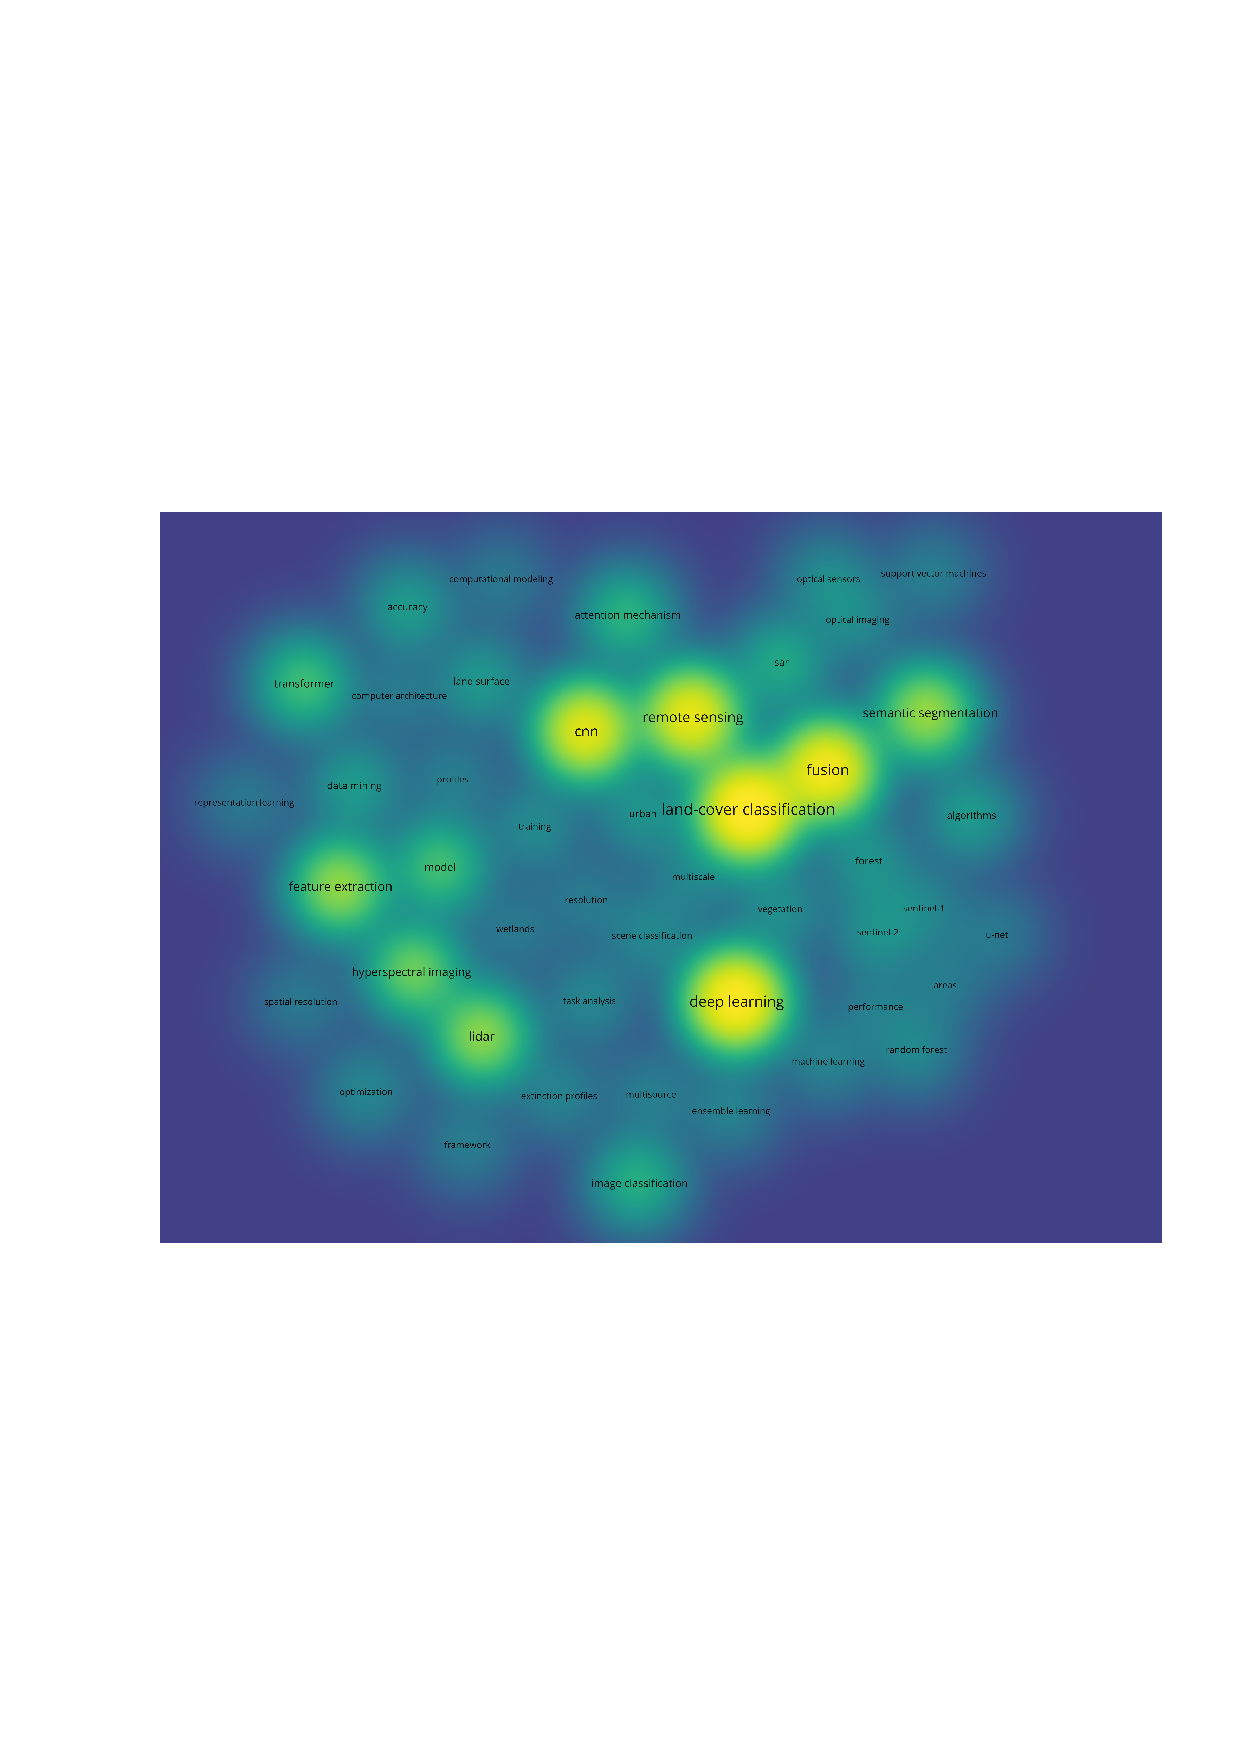
\includegraphics[width=1.0\columnwidth]{Figures/new_Relitu.pdf}
	\caption{Density visualisation of keyword hotspots in the retrieved LULC classification literature.}
	\label{fig:keyword_density}
\end{figure}

Currently, the evaluation of these deep learning fusion models relies heavily on benchmark datasets. The high-density focus on ``hyperspectral imaging'' and ``LiDAR'' in Fig.~\ref{fig:keyword_density} is directly reflected in the dataset utilisation rankings. Our analysis (Fig.~\ref{fig:datasets_ranking}) reveals that Houston (25 studies) and Trento (15 studies) were the most prevalent benchmarks in the included corpus. This concentration highlights the community's reliance on standardised, multimodal data to evaluate the performance of feature-fusion architectures in complex urban and agricultural environments. However, concentration on a few curated datasets limits conclusions about cross-region, large-area, and temporally dynamic mapping.

\begin{figure}[!htbp]
	\centering
	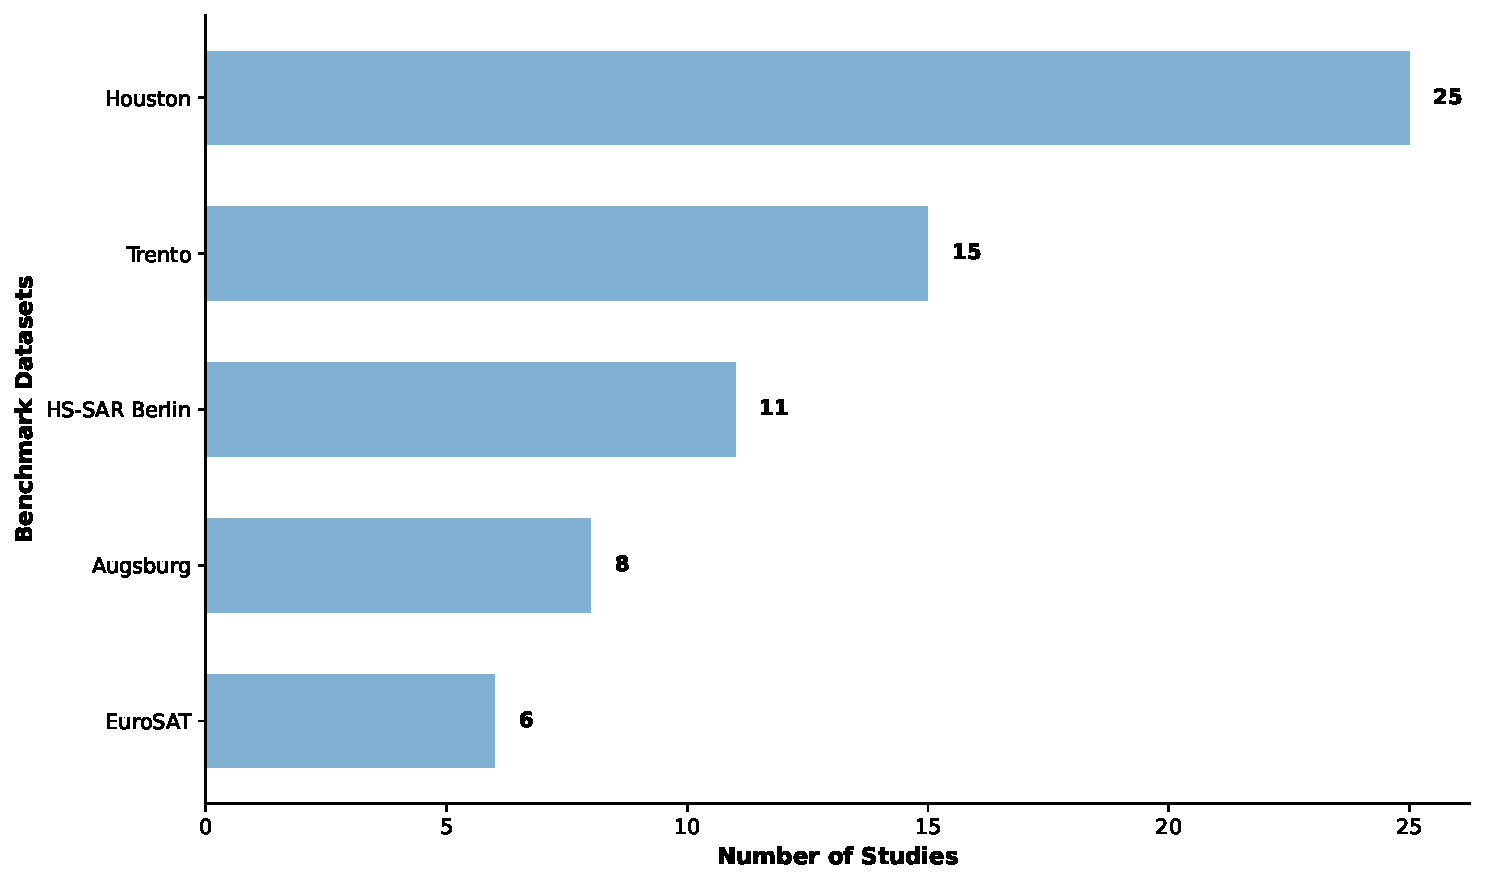
\includegraphics[width=1.0\columnwidth]{Figures/top_datasets_ranking.pdf}
	\caption{Frequency of datasets utilised in the analysed LULC fusion studies. EuroSAT is shown as a corpus-frequency observation; because it contains Sentinel-2 multispectral imagery rather than multimodal data, it is not included in Table~\ref{tab:datasets_detail}.}
	\label{fig:datasets_ranking}
\end{figure}

\begin{table}[!htbp]
	\centering
	\setlength{\belowcaptionskip}{8pt}
	\caption{Technical specifications of representative multimodal benchmark datasets used in LULC classification.}
	\label{tab:datasets_detail}
	\scriptsize
	\setlength{\tabcolsep}{3pt}
	\renewcommand{\arraystretch}{1.25}
	\begin{tabular}{@{} p{1.8cm} p{3.5cm} p{3.2cm} c p{3.5cm} @{}}
		\toprule
		\textbf{Dataset} & \textbf{Modalities (Sensors)} & \textbf{Resolution} & \textbf{Classes} & \textbf{Dimensions (px)} \\ 
		\midrule
		Houston 2013  & HSI (144 bands) + LiDAR      & 2.5 m   & 15 & $349 \times 1905$ \\ 
		Trento        & HSI (63 bands) + LiDAR        & 1.0 m   & 6  & $600 \times 166$ \\ 
		Berlin        & HSI (244 bands) + SAR         & 30 m (HSI); 13--13.9 m (SAR) & 8  & $797 \times 220$ (HSI); $1723 \times 476$ (SAR) \\ 
		Augsburg      & HSI (180 bands) + SAR + digital surface model (DSM) & 30 m (co-registered products) & 7  & $332 \times 485$ \\ 
		MUUFL Gulfport & HSI (64 bands) + LiDAR       & 1 m (co-registered grid) & 11 & $325 \times 220$ \\ 
		\bottomrule
	\end{tabular}
\end{table}

As evidenced by the technical specifications in Table~\ref{tab:datasets_detail}, the integration of heterogeneous data requires different algorithmic strategies. The diversity in spatial resolution and spectral dimensionality across these benchmarks, particularly the HSI and LiDAR combinations in Houston and MUUFL Gulfport, has historically driven the evolution of fusion methodologies.  EuroSAT is retained in Fig.~\ref{fig:datasets_ranking} only as a corpus-frequency observation and is excluded from Table~\ref{tab:datasets_detail} because it contains Sentinel-2 multispectral imagery rather than multimodal observations. Trento, Berlin, Augsburg, and MUUFL specifications follow published benchmark descriptions and the official release \citep{duan2020multilevel,hong2021benchmarks,gader2013muufl,zare2018muufl}.

Driven by this evidence, research typically categorises fusion technologies into three levels: data-level fusion, feature-level fusion, and decision-level fusion, as illustrated in Fig.~\ref{fig:fusion_stages}. These are alternative integration choices rather than a mandatory progression. Hybrid fusion combines explicit integration at two or more levels.

\begin{figure}[!htbp]
	\centering
	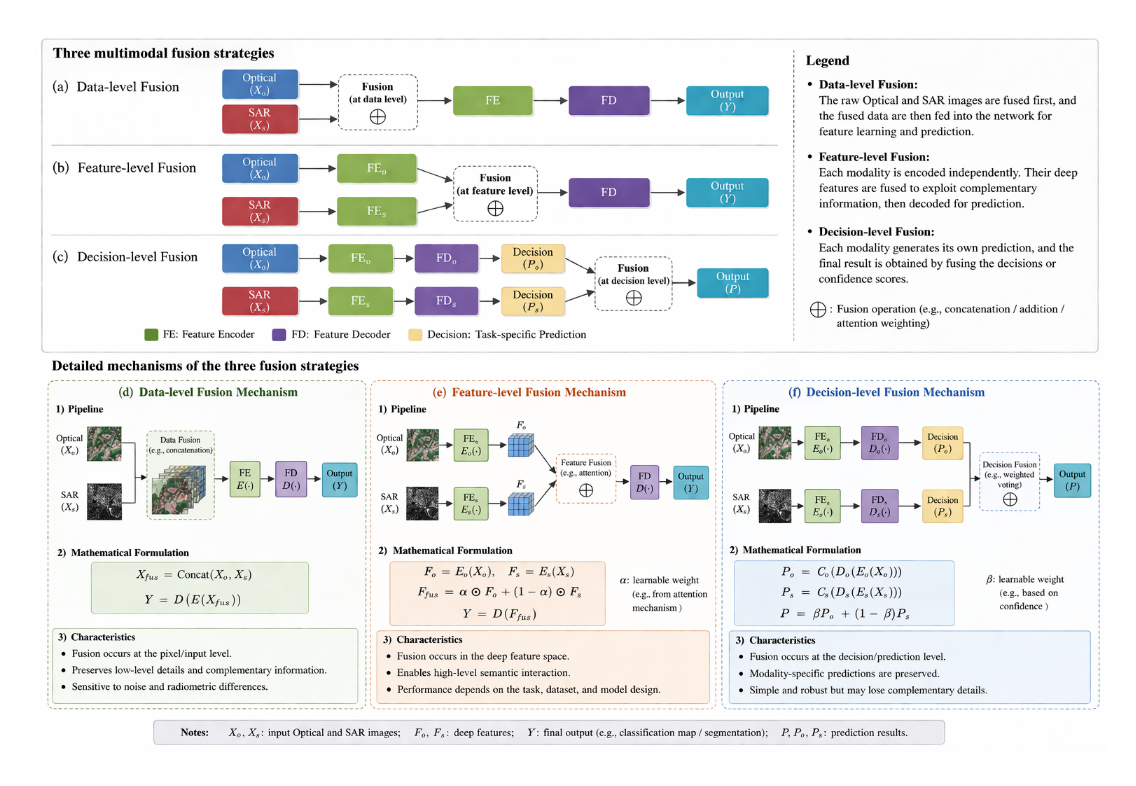
\includegraphics[width=1.0\columnwidth, trim=0 10 0 10, clip]{Figures/Fusion_Picture.pdf}
	\caption{Three principal fusion levels considered in LULC classification: (a) data-level fusion, (b) feature-level fusion, and (c) decision-level fusion. These levels represent alternative design choices rather than a mandatory progression.}
	\label{fig:fusion_stages}
\end{figure}

Table~\ref{tab:fusion_levels} compares the main design and evaluation implications of the four fusion levels. Fusion level is defined by the first stage at which modality-specific streams exchange information; hybrid fusion requires explicit fusion at two or more distinct stages. Representative implementations for each level are identified in the table note. Here $M$ is the number of modalities, $C$ the number of classes, $d_m$ the input width of modality $m$, $N_i$ and $N_j$ the numbers of positions or tokens, and $d$ the latent dimension. The complexity terms describe representative operators rather than complete implementations. Accuracy and measured runtime are not ranked across publications because datasets, hardware, training budgets, and evaluation protocols differ.

\begin{table}[!htbp]
	\centering
	\caption{Design and evaluation considerations for multimodal LULC fusion levels.}
	\label{tab:fusion_levels}
	\footnotesize
	\setlength{\tabcolsep}{2pt}
	\renewcommand{\arraystretch}{1.18}
	\begin{tabular}{@{} >{\raggedright\arraybackslash}p{1.25cm} >{\raggedright\arraybackslash}p{2.90cm} >{\raggedright\arraybackslash}p{3.00cm} >{\raggedright\arraybackslash}p{2.65cm} >{\raggedright\arraybackslash}p{3.65cm} @{}}
		\toprule
		\textbf{Fusion level} & \textbf{Integration and data needs} & \textbf{Training and computation} & \textbf{Key risks} & \textbf{Minimum evidence and suitable conditions} \\
		\midrule
		Data-level & Combines co-registered inputs before representation learning. Grid concatenation requires spatial correspondence and sensor-appropriate normalisation. & Usually trained jointly. Concatenation increases encoder input width to $\sum_m d_m$; cost grows with source count and preprocessing. & Misregistration, acquisition-time mismatch, redundant or noisy bands, and dominance of a high-dimensional source. & Compare each source with concatenation and perturb registration and acquisition time. Most suitable when inputs are accurately aligned and low-level correspondence is important. \\
		\addlinespace[2pt]
		Feature-level & Combines intermediate modality-specific or shared representations. Resampling or learned alignment can accommodate some resolution differences, but semantic correspondence remains necessary. & Uses separate encoders and a fusion module. Dense pairwise cross-attention scales as $O(N_iN_jd)$ in time and $O(N_iN_j)$ in attention memory. & Modality dominance, overfitting, alignment shift, and brittleness to missing or corrupted sources. & Require modality ablation, missing- and misaligned-source stress tests, and a compute-matched late-fusion baseline. Suitable when detailed cross-modal interaction is required. \\
		\addlinespace[2pt]
		Decision-level & Aggregates scores, probabilities, labels, or maps. Feature spaces need not match, but classes and spatial units must be compatible. & Branches may be trained independently. Simple score averaging adds $O(MC)$ operations beyond branch inference. & Miscalibration, correlated errors, incompatible taxonomies, and loss of fine cross-modal interaction. & Report branch performance, error correlation, calibration, and missing-branch tests. Suitable for ensembles and modular sensor pipelines. \\
		\addlinespace[2pt]
		Hybrid & Uses explicit fusion at two or more stages, such as feature interaction followed by score aggregation. & Architecture-dependent and jointly or sequentially trained. Report parameters, floating-point operations, memory, and latency. & Redundant paths, cross-stage co-adaptation, optimisation instability, error propagation, and unclear attribution of gains. & Require stage-wise ablation and compute-matched single-level baselines. Suitable when both fine cross-modal interaction and modular prediction are needed. \\
		\midrule
		\multicolumn{5}{@{}>{\raggedright\arraybackslash}p{13.45cm}@{}}{\scriptsize \textit{Note.} Representative implementations comprise data-level fusion \citep{6,37}, feature-level fusion \citep{23,41,zhang2023multimodal}, decision-level fusion \citep{55}, and hybrid feature--decision fusion \citep{hang2020coupled}. These references illustrate the respective fusion levels; the risks and minimum-evidence recommendations are the authors' synthesis and are not attributed in full to any individual study. Attention-complexity estimates are based on \citet{vaswani2017attention}.} \\
		\bottomrule
	\end{tabular}
\end{table}

The entries in Table~\ref{tab:fusion_levels} are conditional design expectations rather than universal rankings. The cited studies illustrate implementations of particular fusion levels but do not establish that one level is uniformly more accurate, efficient, robust, or interpretable. In hyperspectral classification, spatially overlapping sampling can inflate performance estimates \citep{liang2017sampling}; comparisons should therefore use identical preprocessing and geographically disjoint splits where possible. Temporal leakage, class imbalance, label uncertainty, and inconsistent preprocessing are likewise evaluation-wide threats. Comparative studies should include the strongest single-modality model, simple input concatenation, simple score averaging, and a parameter- or compute-matched baseline where applicable.

\FloatBarrier

\subsection{Data-Level Fusion}
Data-level fusion, often referred to as pixel-level or raw-level fusion, involves the direct integration of co-registered multimodal data sources, such as optical imagery, LiDAR-derived products, and SAR \citep{57}. Bibliometric trends from 2016 to 2025 indicate that while keywords such as ``LiDAR'' and ``remote sensing'' occur frequently in the retrieved corpus \citep{38, 39}, studies investigate the synergy of these sensors to address individual spectral or structural limitations. The prominent status of LiDAR is attributed to its capacity to provide high-precision 3D coordinates and vegetation structure information, which can complement optical imagery from sensors like Sentinel-2; cloud-penetrating observations are provided by SAR rather than LiDAR \citep{40}.

Despite its foundational importance, data-level fusion faces persistent technical bottlenecks, particularly in multi-source spatial registration and heterogeneous noise suppression \citep{41}. Statistical models of heterogeneous SAR returns illustrate the need to account for sensor-specific noise \citep{58}. High-quality fused inputs can support subsequent feature extraction by CNNs, Transformers, and state-space models, but alignment alone does not ensure improved classification. Registration accuracy, source-specific noise, sensor complementarity, and training conditions must be considered when preparing ``model-ready'' multimodal inputs \citep{23,cao2020urban}.


\clearpage
\subsection{Feature-Level Fusion and Technical Evolution}

\begin{table}[htb!]
	\centering
	\setlength{\belowcaptionskip}{5pt}
	\caption{Comparison of deep learning models for feature-level fusion in LULC.}
	\label{tab:comparison_models}
	\scriptsize
	\setlength{\tabcolsep}{2pt}
	\renewcommand{\arraystretch}{1.4} % 稍微降低基础缩放，依靠 addlinespace 来提供自然的段落间隔
	\begin{tabular}{@{} >{\raggedright\arraybackslash}p{1.9cm} >{\raggedright\arraybackslash}p{2.25cm} >{\raggedright\arraybackslash}p{2.8cm} >{\raggedright\arraybackslash}p{3.0cm} >{\raggedright\arraybackslash}p{3.0cm} @{}}
		\toprule
		\textbf{Method} & \textbf{Role in Fusion} & \textbf{Advantages} & \textbf{Disadvantages} & \textbf{Recent Trend} \\ 
		\midrule
		CNN & Backbone for local feature extraction. & Excels at texture/edge capture. & Limited receptive field; long-range interaction requires additional depth or modules. & Hybrid CNN-Transformer architectures. \\ 
		\addlinespace[0.8em] % 用优雅的空隙代替硬邦邦的内侧横线
		
		Transformer & Global feature interaction via self-attention. & Direct interaction between tokens; can support cross-modal fusion. & Dense attention has quadratic token-pair cost; data demand is task-dependent. & Windowed attention (Swin); multi-level fusion (SoftFormer). \\ 
		\addlinespace[0.8em]
		
		Attention Mechanisms & Adaptive weight regulation module. & Can suppress noise and enhance key features; weights are not necessarily explanations. & Increases computational overhead. & Cross-modal attention; alignment still requires evaluation. \\ 
		\addlinespace[0.8em]
		
		Mamba & Sequence and long-range modelling. & Theoretically linear sequence scaling; total cost is implementation-dependent. & Early stage; limited 2D multimodal and cross-region validation. & Development of spatiotemporal frameworks (e.g., Geo-Mamba). \\ 
		\bottomrule
	\end{tabular}
\par\smallskip\begin{minipage}{0.98\textwidth}\scriptsize\textit{References by method:} CNN \citep{2, 8, 29, 56}; Transformer \citep{7, 35, 36, bazi2021vision, liu2024softformer}; Attention Mechanisms \citep{46, 47, zhang2023multimodal}; Mamba \citep{5,49,53}.\end{minipage}
\end{table}
\FloatBarrier

Feature-level fusion integrates abstract features at the intermediate layers of a model (such as feature maps extracted via a CNN or Transformer), with a balance between information preservation and computational efficiency that depends on the model and task. Within the retrieved corpus, bibliometric analysis reveals that ``CNN'', ``deep learning'', and ``feature extraction'' are among the highest-frequency keywords, alongside emerging terms such as ``Transformer'', ``attention mechanism'', ``representation learning'', and ``semantic segmentation''.

DL: DL provides an end-to-end framework for feature-level fusion, enabling the unified implementation of automated feature extraction and decision-making. In LULC research, DL models automatically mine multi-dimensional spectral, spatial, and textural features, reducing dependence on manual feature engineering. This supports the use of feature-level fusion in the reviewed studies \citep{42, 43}. Notably, the study ``Deep Learning Earth Observation Classification Using ImageNet Pretrained Networks'' \citep{28} had a TGCS of 492 at the time of data collection, reflecting the intense research focus on DL-driven methodologies.

\medskip % 增加段落间距
CNN: CNNs served as the core tools for early feature-level fusion. They excel at capturing local spatial features, such as building textures and vegetation patch structures. By extracting and fusing local features from multi-source data (e.g., optical and SAR) through channel concatenation or weighted summation, CNNs can improve classification accuracy, depending on data alignment, training, and evaluation conditions \citep{41}.

\medskip
Transformer: This architecture has seen a rapid surge in popularity in the retrieved literature. The 2023 study ``Extended Vision Transformer (ExViT) for Land Use and Land Cover Classification'' \citep{36} achieved a TGCS of 312 at the time of data collection. By utilising self-attention mechanisms, Transformers can capture long-range spatial dependencies beyond local convolutional receptive fields, although benefits depend on training data, tokenisation, spatial scale, and computational resources \citep{45}.

\medskip
Feature Extraction and Attention Mechanisms: These represent the core technical phases of fusion. Feature extraction is the prerequisite, converting raw multi-source data (optical, SAR, LiDAR) into discriminative abstract representations. Meanwhile, the attention mechanism automatically learns weights to prioritise features most relevant to LULC tasks, such as building edges or specific vegetation signatures \citep{46, 47}. Attention weights alone do not establish causal explanations; modality ablation and matched fusion baselines are needed to assess their contribution.

\medskip
Semantic Segmentation: This is a prevalent application scenario for feature fusion. LULC research requires not only type identification but also the precise delineation of spatial boundaries. By integrating complementary information, feature fusion produces refined segmentation results for roads, buildings, and green spaces, with results dependent on resolution, label definitions, and evaluation design \citep{45, 48}.

Of particular note is the rapid emergence of the \textbf{Mamba} architecture. Although it currently appears with low frequency (only 4 times) in the keyword co-occurrence network, its role as a backbone for LULC fusion remains under evaluation. Dense Transformer self-attention permits long-range interaction, but its pairwise interaction cost grows quadratically with token count. In contrast, Mamba introduces a \textit{Selective Scan} mechanism \citep{53}, with theoretically linear scaling in sequence length; end-to-end cost also depends on spatial scanning, encoders, and implementation. Recent studies, such as ``Geo-Mamba'' \citep{49} and ``Semi-Mamba'' \citep{51}, illustrate Mamba's feasibility, not a demonstrated solution to the accuracy-efficiency bottleneck. Further multimodal fusion implementations have also been reported \citep{5,52}. However, as an architecture proposed in late 2023, its application in LULC remains in its infancy and requires further empirical validation across 2D multimodal, cross-region, and cross-sensor settings.

In summary, feature-level fusion has developed into diverse technical lineages. To clearly illustrate the positioning and evolution of different deep learning architectures, Table~\ref{tab:comparison_models} compares the characteristics of mainstream models and key components. These approaches offer different local, long-range, and computational properties; their relative suitability depends on the task and evaluation protocol.


\subsection{Decision-Level Fusion}
Decision-level fusion, also known as late fusion, represents a high-level integration strategy where independent classification outputs from multiple sub-models are combined to reach a final consensus \citep{55}. Ensemble learning and voting strategies provide methodological foundations for this stage \citep{55}. Despite its foundational role in traditional machine learning, our analysis shows that it occurs less frequently than feature-level approaches in the archived fusion-content subset, without implying inferior performance.

The primary limitation of decision-level fusion lies in its ``information decoupling'' nature: by processing each data source independently, it may not capture low-level complementary relationships and cross-modal correlations available to jointly learned representations \citep{6}. However, combining independent models permits modular replacement and separate validation. Decision fusion can support uncertainty estimation and multi-model verification \citep{55,kampffmeyer2018urban}, but correlated branch errors and poorly calibrated probabilities can limit its value. Missing-modality robustness requires an aggregation rule designed for variable source availability; it is not guaranteed by late fusion alone.


\subsection{Learning Strategies Beyond Architecture Design}

The preceding sections have examined fusion at the data, feature, and decision levels and the architectures used to implement it. Beyond these design choices, learning strategies also influence the effectiveness of multimodal LULC classification. The learning strategy determines how supervision is obtained, how modalities are aligned, and whether a trained model remains reliable outside the training distribution. Self-supervised pre-training can exploit unlabelled Earth observation archives by reconstructing masked inputs or learning invariant representations before task-specific fine-tuning. For example, SatMAE adapts masked autoencoding to multispectral and temporal satellite imagery, illustrating how spectral groups and acquisition time can be incorporated into pre-training rather than treated as ordinary colour channels \citep{cong2022satmae}. Such pre-training may reduce label requirements, but improvements must be tested against training from scratch under identical data, augmentation, and compute budgets.

Federated learning can support training across separate clients without centralising their raw data; FedDiff investigates diffusion-driven learning for multiple modalities and clients \citep{li2024feddiff}. Domain adaptation and domain generalisation address changes in geography, season, sensor, resolution, and class prevalence. Adaptation methods use information from a target domain, whereas generalisation methods aim to perform on unseen domains without target-domain training. Both require spatially separated and temporally separated evaluation; random patch splits can overestimate transfer when nearby samples share landscape context. Semi-supervised learning can combine limited labels with unlabelled observations, while class-balanced sampling, cost-sensitive objectives, and calibrated uncertainty estimates can address rare classes and ambiguous boundaries. For multimodal systems, evaluation should also include missing-source, corrupted-source, and asynchronous-acquisition conditions rather than assuming that every modality is available and perfectly registered \citep{kampffmeyer2018urban}.

Efficiency is likewise a learning and deployment issue, not merely an architectural label. A recent long-term wetland study used lightweight attention-conditional convolution to reduce model cost while retaining task-specific temporal modelling \citep{yin2026lacc}. Lightweight land-target detection \citep{wang2024cgbiyolo} and dual-branch infrared target enhancement \citep{wang2025dabfnet} provide potentially transferable ideas for compact backbones and branch interaction, but their detection objectives differ from LULC classification. Their reported results therefore cannot be used as direct evidence of classification performance.

Recent applications illustrate several adjacent design directions: global-scale SAR inference for iceberg detection \citep{xie2026iceberg}; Transformer--hypergraph aggregation and cross-view filtering for unmanned aerial vehicle (UAV) localisation \citep{huang2026htgl,su2026cpfl}; hybrid physical and data-driven retrieval of land-surface temperature and emissivity \citep{wang2024lst}; and the coupling of compressed sensing with deep learning for polarisation super-resolution \citep{wu2026polarization}. These tasks are not LULC classification benchmarks. They are cited to identify transferable questions---global deployment, physics-aware learning, efficient feature aggregation, and sensing--model co-design---that require separate validation in LULC settings.

\subsection{Remote Sensing Foundation Models and Multimodal Pre-training}

Remote sensing foundation models are generally understood as models pre-trained on large and diverse Earth observation corpora and subsequently adapted to multiple downstream tasks \citep{cong2022satmae,liu2024remoteclip}. They differ from a task-specific pre-trained network in intended breadth, scale, and transfer, although the boundary is not always sharp. Multimodal foundation models seek representations that can connect different sensors or data types, while vision--language models additionally align imagery with text. This terminology distinguishes the model class from the broader process of multi-source fusion.

Current work spans several complementary approaches. SatMAE demonstrates self-supervised pre-training for temporal and multispectral satellite data \citep{cong2022satmae}. RemoteCLIP aligns remote sensing imagery and language, enabling zero-shot or transfer-oriented use of semantic text supervision \citep{liu2024remoteclip}. Foundation-model-based multimodal classification has also been investigated for heterogeneous remote sensing data \citep{he2024foundation}, and a unified multimodal fine-tuning framework has been evaluated for remote sensing semantic segmentation \citep{ma2025multimodal}. Collectively, these studies indicate that pre-training can support transferable representations, but they do not establish one universal model or adaptation strategy for LULC classification.

Several unresolved issues limit stronger conclusions. Pre-training archives are geographically and temporally imbalanced; sensor, resolution, and label taxonomies differ across downstream datasets; and large models impose substantial training and inference costs. Apparent transfer gains can also be inflated by geographic overlap or near-duplicate imagery between pre-training and evaluation data. Future comparisons should disclose pre-training sources, check spatial and temporal leakage, match compute budgets, report per-class and calibration metrics, and compare full fine-tuning with parameter-efficient and frozen-encoder baselines. Multimodal evaluation should further test whether gains persist when a source is missing, degraded, or acquired at a different time.

\section{Challenges in LULC Studies}
Based on the bibliometric analysis, a distinct contrast emerges: while algorithmic keywords such as \textit{Deep Learning}, \textit{Transformer}, and \textit{Fusion} occur frequently in the retrieved corpus, terms related to \textit{Data Quality}, \textit{Uncertainty Analysis}, and \textit{Error Propagation} remain relatively marginalised. This contrast motivates discussion of data reliability, although keyword frequency does not measure the practical importance of a problem. In LULC studies, data reliability is paramount; it serves as the foundation for deep learning models. However, the acquisition and integration of high-quality data still face severe challenges.

\subsection{Data-Level Challenges}

In the following, we categorise the challenges associated with the data in four aspects:

\begin{enumerate}
	\item \textbf{Intrinsic Quality and Uncertainty:} Raw data quality is a persistent issue. Optical imagery is frequently obscured by cloud cover and lighting variations; SAR imagery suffers from inherent speckle noise; and LiDAR point clouds often contain outliers. Errors in raw data can be propagated or amplified by deep learning models during feature extraction, leading to distorted classification results. Uncertainty in land-use inputs can also affect downstream conclusions across spatial scales \citep{li2026landuncertainty}.
	\item \textbf{Spatiotemporal Inconsistency:} This represents a core physical barrier to effective fusion. Optical, SAR, and LiDAR data possess natural discrepancies in spatial resolution, observation angles, and imaging times. Residual sub-pixel offsets and acquisition-time differences can lead models to learn incorrect feature correspondences. Furthermore, radiometric drift in long-term monitoring may trigger ``pseudo-change'' misinterpretations. Acquisition dates, registration accuracy, resampling, and sensitivity to temporal offsets should therefore be reported.
	\item \textbf{Scarcity and Imbalance of High-Quality Annotations:} The development of supervised learning is bottlenecked by the lack of labelled samples \citep{56}. LULC tasks require precise pixel-level annotation, which demands extensive expert knowledge and is time-consuming. In complex mixed-pixel regions, subjective inconsistencies in manual labelling can lead to model overfitting, limiting applications in large-scale scenarios. Rare classes and inconsistent label taxonomies can also bias overall accuracy towards common classes; per-class results and class-balanced evaluation are needed.
	\item \textbf{Limited Benchmark Representativeness:} Houston, Trento, MUUFL Gulfport, Berlin, and Augsburg are valuable controlled benchmarks, but their geographic extent, sensor combinations, and class schemes do not represent every operational setting. Results from random within-scene splits should not be assumed to transfer to new regions, seasons, or sensors. Cross-region and temporal hold-out evaluation is needed to measure this gap.
\end{enumerate}


\subsection{Algorithm-Level Challenges}

In the following, we categorise the challenges associated with algorithms into four aspects, setting the stage for the subsequent discussion of potential remedies.


\begin{enumerate}
	\item \textbf{Semantic Gap in Multimodal Features:} There is a distribution difference between the spectral features of optical imagery and the structural features of SAR/LiDAR. Simple channel concatenation or weighted summation does not itself provide adaptive feature alignment. This makes it difficult to fully exploit the complementarity between heterogeneous data, potentially losing critical information.
	
	\item \textbf{Lack of Interpretability:} CNNs and Transformers are often viewed as black boxes. It is difficult to intuitively reveal the physical mechanisms behind classification decisions, for instance, whether the model relies on LiDAR height info or optical texture. This opacity makes it challenging to quantify the contribution of different modalities to LULC predictions, weakening the persuasiveness of geographical explanations. Modality ablation, counterfactual masking, attribution stability, and probability calibration provide complementary evaluation evidence.
	
	\item \textbf{Insufficient Generalisation:} Random within-scene training/test splits do not establish generalisation to new regions. However, real-world LULC scenarios (e.g., from urban to mountainous areas) exhibit significant \textit{domain shift}. Models trained in specific regions often suffer performance degradation when migrated to heterogeneous new areas or time periods, hindering the goal of ``train once, apply globally''. Geographically and temporally disjoint tests are therefore needed to measure transfer. 
	\item \textbf{Efficiency and Operational Constraints:} Model size, memory use, latency, energy consumption, and preprocessing cost affect whether a method can be deployed at national or global scale. Theoretical linear sequence scaling in state-space models is promising, but end-to-end cost also includes multimodal encoders, image tiling, data transfer, and post-processing. Comparisons should report parameters, floating-point operations or measured latency, memory, hardware, input size, and accuracy under the same protocol.
\end{enumerate}


\section{Reproducibility and Open Science}

Supporting materials for this review are available at \url{https://github.com/cj1102/DL-LULC-Fusion-Review}. They include the 261-record bibliometric input, search and cleaning documentation, retained network outputs, the fusion-coding protocol, and the 163 record-level fusion assignments. Detailed methodological notes document corpus reconciliation and the evidence and limitations associated with the retained VOSviewer settings.

\section{Conclusion}
This review uses bibliometric and network analyses of 261 WoSCC publications (2006--2025) to examine DL and multi-source data fusion in LULC classification. Publication activity increased from 2016 to 2025 within this intersection. The search required both DL and fusion terms, so it cannot establish that DL replaced traditional machine learning or that fusion became dominant across LULC research. China and Germany rank among the top three by publication count, TLCS, and TGCS within the corpus; these metrics do not measure national innovation capacity.

Within the selected corpus, feature-level fusion combines complementary spectral, structural, and textural information from optical imagery, SAR, and LiDAR; robustness and versatility depend on alignment, sample availability, computation, and application. CNNs extract local features, while Transformers and attention mechanisms support global context aware modelling. State-space models such as Mamba offer favourable theoretical sequence scaling, but their 2D multimodal and cross-region performance remains insufficiently validated.

Data reliability and model robustness remain bottlenecks. Spatiotemporal sensor inconsistencies introduce ``pseudo-changes''. The ``black box'' nature of models limits their use in decisions requiring geographical interpretability. Dependence on large labelled datasets hinders generalisation where ground truth is scarce. Small benchmarks alone cannot validate global or temporally dynamic mapping.

Future research should prioritise explainable fusion models that quantify feature contributions and connect DL outputs with geographical process understanding. Remote sensing foundation models may support few-shot adaptation or zero-shot transfer with scarce high-quality annotations, but geographic bias, leakage risks, computational cost, and cross-region reliability require evaluation. Data governance and harmonisation should improve registration and normalisation to address sensor discrepancies and provide ``model-ready'' data with fewer spatiotemporal inconsistencies. Further priorities include uncertainty calibration, domain adaptation and generalisation, continual learning, and standardised geographic and temporal evaluation protocols.

DL and multi-source fusion have expanded LULC classification approaches. Further advances require a balance between model accuracy, physical interpretability, and cross scene generalisation to provide reliable, evidence-based scientific support for global environmental monitoring and sustainable land resource management.


\bibliographystyle{apacite}
\bibliography{interactapasample}

\end{document}
